\documentclass[a4paper, 11pt, titlepage, twoside]{article}

\usepackage{preamble}

\begin{document}
%Canviem el nom de l'apartat Referències per ``Bibliografia''

%Portada

%%CANVIEU L'ESPAI VERTICAL ENTRE ELEMENTS SEGONS LA LLARGADA DEL TÍTOL
\begin{titlepage}
    {\centering
    {\Huge Master Thesis}\\
    \vspace{5mm}
    {\Large \textbf{Double MSc Degree in Industrial Engineering and Energy Engineering}}\\
    \vspace{20mm}
    \Huge \textbf{Dynamic Simulation and Stability Analysis of Power Systems: Development of RMS and EMT Tools within VeraGrid at eRoots}\\
    \vspace{10mm}
    \Large{January 2026}\\  %Data de la darrera complicació, si voleu posar una data fixa, escriviu-la aquí
    }
    \vspace{25mm}
    \hspace{2mm}
    \begin{tabular}{l@{ } l}
        \vspace{5mm}
        \Large \textbf{Author:} & \hspace{3mm} \Large{Maria Sans Esqué} \\
        \vspace{5mm}
    \Large\textbf{Supervisors:} & \hspace{3mm} \Large{Vinícius Albernaz Lacerda} \\
                                & \hspace{3mm} \Large{Josep Fanals i Batllori} \\

    \end{tabular}\par
    \vspace{10mm}
    {\centering
    
\includegraphics[scale=0.3]{./Icones-ETSEIB-UPC/ETSEIB.png}\\
    {\Large Escola Tècnica Superior \\ d'Enginyeria Industrial de Barcelona}\\
    \vspace{3mm}
    
\includegraphics[scale=0.4]{./Icones-ETSEIB-UPC/UPC.PNG}
    \par
    }
    \end{titlepage}

%Pàgina en blanc
\clearpage
\thispagestyle{empty}
\null\newpage 

%iniciem la numeració des del Resum
\pagenumbering{arabic}

\section*{Abstract}\label{Abstract}
\input{Chapters/Abstract}
\cleardoublepage
\section*{Resumen}\label{Resumen}


\cleardoublepage
\section*{Resum}\label{Resum}





\cleardoublepage

\tableofcontents

\newpage
\listoffigures

\newpage
\begingroup
\setlength{\parskip}{0pt}
\listoftables %Opcional
\endgroup

\setlength{\abovedisplayskip}{5pt} % Equation spacing adjusted
\setlength{\belowdisplayskip}{5pt} % Equation spacing adjusted

\section*{Glossary}
\addcontentsline{toc}{section}{Glossary}
\subsection*{Symbols}
\begin{tabular}{l@{\hspace{1.95cm}} l}
  $\bm{\theta}$ & Voltage angle vector \\
  $\lambda$ & Eigenvalue \\
  $\zeta$ & Damping ratio \\
  $\bm{\omega}$ & Angular frequency vector \\
  $\bm{A}$ & State matrix \\
  $\bm{B}$ & Input matrix \\
  $\bm{C}$ & Output matrix \\
  $\bm{D}$ & Feedthrough matrix \\
  $\bm{x}$ & State vector \\
  $\bm{u}$ & Input vector \\
  $\bm{y}$ & Output vector \\
  $\tau$ & Time constant \\
  
  
 
\end{tabular}


\subsection*{Acronyms}
\begin{tabular}{l@{\hspace{1cm}} l}
  AC & Alternating Current \\
  CIG & Converter-interfaced Generation \\
  DAE & Differential Algebraic Equation\\
  DC & Direct Current \\
  EEA & European Environment Agency\\
  EMT & Electro Magnetic Transient\\
  ETSEIB & Escola Tècnica Superior d'Enginyeria Industrial de Barcelona\\
  GUI & Guided User Interface\\
  HVAC & Heating Ventilation and Air Conditioning \\
  IBR & Inverter-Based Resources \\
  ICAEN & Institut Català de l'Energia \\
  IGE & Induction Generator Effect\\
  LCA & Life Cycle Assessment \\
  ODE & Ordinary Differential Equation \\
  PF & Participation Factor\\
  PSCAD & Power Systems Computer Aided Design\\
  RMS & Root Mean Square\\
  SFA &Shifted Frequency Analysis\\
  SPT & Singular Perturbation Theory\\
  SSCI & Subsynchronous Control Interaction\\
  SSR & Subsynchronous Resonance\\
  TDS & Time Domain Simulation\\
  
\end{tabular}\par
\newpage

\section*{Preface}
\addcontentsline{toc}{section}{Preface}
\input{Chapters/Preface.tex}
\newpage

\section{Introduction}\label{Introduction}
%INTRODUCTION
\subsection{Motivation}

...

\subsection{Objectives}

This thesis is part of the ongoing development of the dynamic simulation framework, 
with a focus on extending its capabilities to include small-signal stability analysis and foundational electromagnetic transient (EMT) modeling. 
The work is carried out within the Veragrid environment, where new modules and methodologies are being implemented. 
The main goal is to equip Veragrid with advanced tools for studying the dynamic behavior of power systems, integrating symbolic modeling, numerical routines,
and graphical interfaces for analysis and visualization.

\subsubsection*{General Objectives}

To develop and validate advanced methodologies for dynamic simulation and stability analysis of power systems by incorporating small-signal stability techniques and foundational EMT modeling, fully integrated into the Veragrid environment.

\subsubsection*{Specific Objectives}

\begin{itemize}
    \item To develop the small-signal analysis module for RMS models, including the formulation and linearization of differential-algebraic equations at the operating point, the computation of eigenvalues and participation factors from the Jacobian matrix, and its integration into Veragrid’s graphical interface.
    \item To implement the foundational components for EMT simulation, modeling transmission lines and system elements in the abc domain, applying discretization techniques such as the Dommel algorithm and alternatives like the 2S-DIRK method, and validating the EMT solver using benchmark systems compared against commercial tools such as PSCAD.
    \item To extend symbolic system formulation to support custom models and control schemes, improving numerical routines, and ensuring consistent initialization of dynamic studies.
    \item To validate the developed methodologies through case studies, continuously comparing results with commercial tools to ensure model reliability and correctness.
\end{itemize}




\subsection{Scope}

This thesis is part of the ongoing development of Veragrid, a leading software platform for power system planning and simulation. 
The work focuses on improving dynamic simulation tools for modern grids, particularly in the context of small-signal stability and electromagnetic transient (EMT) modeling.
Over a nine-month period—from September 2025 to May 2026—the project aims to build essential components that support symbolic formulation, numerical validation,
and integration with existing simulation environments. 

The first major area of focus is the implementation of small-signal stability analysis using RMS-based state-space models.
This includes the computation of eigenvalues and participation factors, symbolic reduction of system equations,
and integration of these routines into the VeraGrid graphical interface.
The goal is to provide researchers and engineers with intuitive and accurate tools for identifying dominant modes and assessing system stability under varying conditions.

The second area involves the development of a foundational EMT solver in the abc domain. This includes modeling transmission lines and components,
implementing discretization techniques such as the Dommel algorithm and two-stage diagonally implicit Runge-Kutta (2S-DIRK) methods,
and benchmarking solver performance against commercial tools like PSCAD. Although the EMT module is not intended to be exhaustive,
it serves as a proof of concept for future expansion and integration.

All development is conducted in Python, with an emphasis on code quality, symbolic computation, and reproducibility.
The thesis also includes continuous benchmarking and validation using real-world data, including industrial cases.
Technical supervision is provided by the eRoots team, ensuring alignment with architectural standards and long-term project goals.

\subsection{Structure of the document}

llistar tot jeje

\subsection{State of the art}

sdfsfgsfd

\subsection{Veragrid}

VeraGrid is a comprehensive software platform for power system planning and simulation, developed to offer both technical accuracy and accessibility. 
It integrates a wide range of analytical and optimisation tools, covering everything from traditional steady-state analyses to advanced planning functions 
that address the challenges of modern electrical grids. Its capabilities include conventional studies such as power flow, short-circuit, and contingency analyses, 
as well as linear and non-linear optimisation modules used for operational decision-making and long-term investment assessment. Many of these functions are based on 
established industry standards, while others are the result of ongoing research and innovation, designed to push the boundaries of what is possible in open and high-performance 
grid modelling.

\begin{figure}
  \centering
  
\includegraphics[width=0.8\linewidth]{figures/VeraGrid_banner.png}
  \caption{VeraGrid banner. \textit{Source: VeraGrid documentation \cite{veragrid}.}}
  \label{fig:VeraGrid_banner}
\end{figure}

The development of VeraGrid began in 2015 with a clear objective: to create a robust programming library supported by a user-friendly interface. 
This pragmatic vision led to a unique ecosystem where reliability and simplicity coexist with scientific rigour. Over the years, the platform has evolved through a combination 
of commercial projects, academic collaborations, and internal research initiatives, ensuring that its algorithms and methods remain both practical and forward-looking. 
Some of its innovations emerged from the need to address real-world industrial requirements, while others stemmed from curiosity and the exploration of new computational paradigms.

VeraGrid serves a wide audience. For professionals, it provides transparent, efficient, and reproducible tools that enable detailed grid analysis and operational planning. 
For researchers, it represents an open and validated environment capable of integrating experimental algorithms and comparing methodologies. For educators and students, 
it offers a pedagogical platform that connects theoretical concepts with practical, industry-grade implementations. This versatility allows VeraGrid to act as a bridge between 
academia, industry, and future generations of engineers.

Beyond conventional functionalities, VeraGrid includes an extensive set of features designed for modern power systems. 
These include a multi-layered architecture for both usability and computational efficiency; an AC/DC generalised power flow engine that supports hybrid 
grids and converter-based systems; short-circuit and fault analysis modules that incorporate converter control logic; and a suite of optimal power flow, expansion planning, 
and investment analysis tools. The platform also integrates time-series simulation capabilities for renewable energy forecasting, storage operation, and market coupling, 
enabling comprehensive scenario-based studies. 

Thanks to its open-core design, VeraGrid can be easily extended and interfaced with external tools, ensuring interoperability and adaptability to specific project needs. 
It stands not only as a software product but as a complete analytical framework that evolves alongside the energy transition, enabling engineers, researchers, and institutions 
to model, plan, and optimise electrical networks with transparency and scientific depth.

\begin{figure}
  \centering
  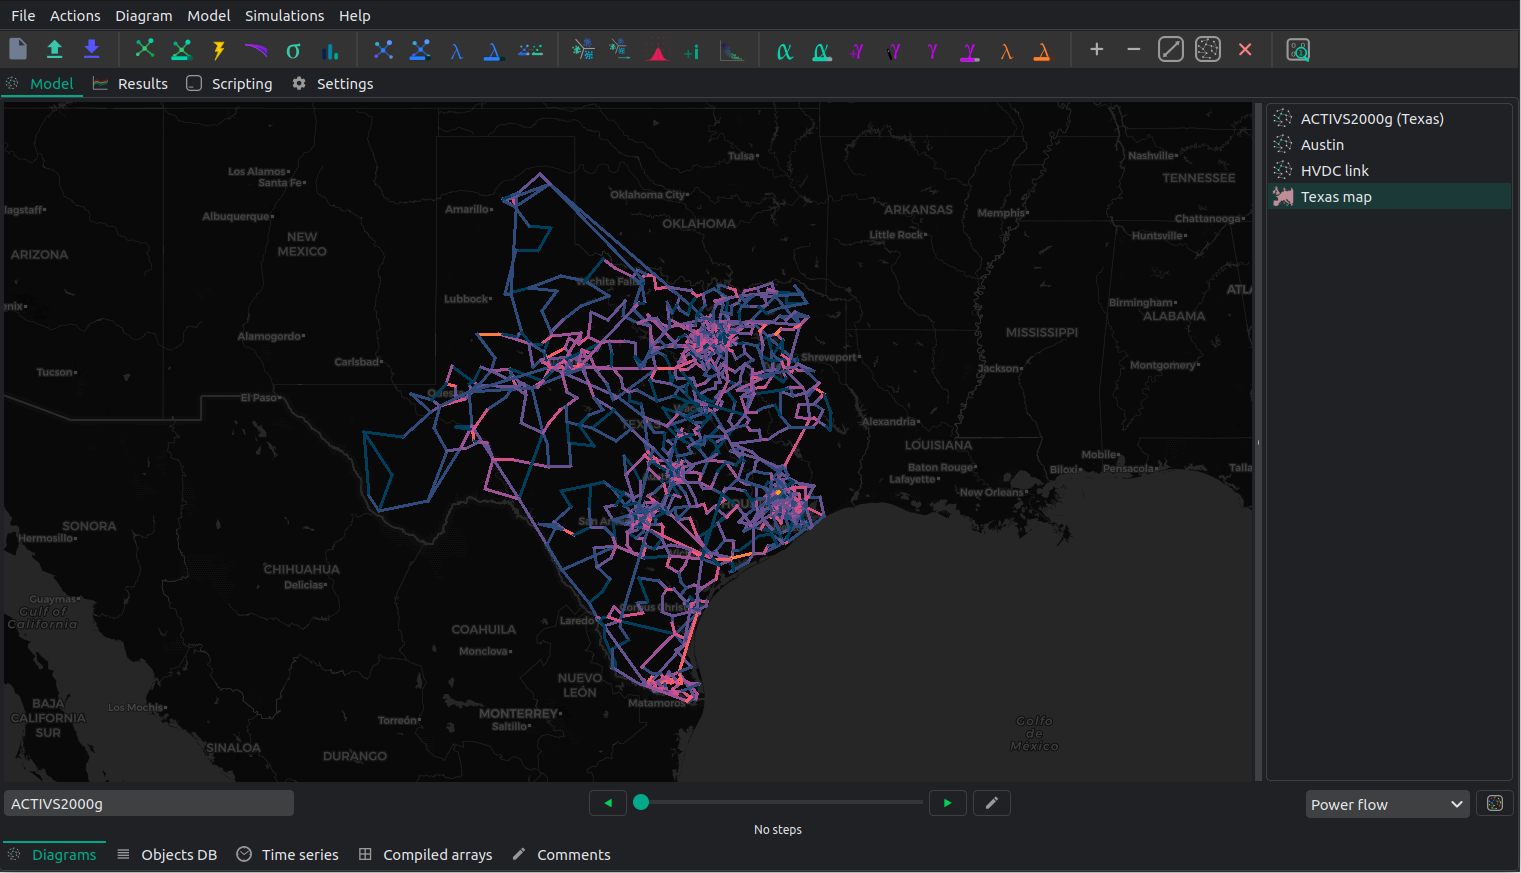
\includegraphics[width=0.8\linewidth]{figures/VeraGrid_main_page.png}
  \caption{VeraGrid main page. \textit{Source: VeraGrid documentation \cite{veragrid}.}}
  \label{fig:VeraGrid_main}
\end{figure}


\subsection{Previous requirements}

Before starting this thesis, it is necessary to have a solid understanding of power system dynamics, numerical methods for differential equations,
and programming in Python. Moreover, this section outlines specific theoretical background on the dynamic simulation of power systems, symbolic formulation and
differential-algebraic equations (DAEs). 

\subsubsection{Dynamic framework in Veragrid}

dfdg

\subsubsection{Symbolic formulation}

ewstrw

\subsubsection{Differential-Algebraic Equations (DAEs)}

CHECK!!

In many dynamic systems, including power systems, one encounters not only purely differential equations but also algebraic constraints linking the state
variables. Such systems are naturally represented by differential-algebraic equations (DAEs). Formally, a DAE is an equation of the form: 

\begin{equation}
  F\bigl(\dot{x}(t),\, x(t),\, y(t),\, t\bigr) = 0
\end{equation}


where $x(t)\in \mathbb{R}^n$ are the differential (dynamic) variables, $y(t)\in \mathbb{R}^m$ are algebraic variables, and the function
 $F$ encodes both the differential and algebraic relations. 
In contrast to an ordinary differential equation (ODE), not all derivatives \(\dot x\) can be explicitly solved from the system because some variables appear only 
algebraically(without derivative) \cite{PolitoDAE}.  

One common formulation is the so-called semi-explicit DAE of index 1:  
\begin{equation}
\begin{cases}
\dot x = f\bigl(x,\,y,\,t\bigr) \\
0 = g\bigl(x,\,y,\,t\bigr)
\end{cases}
\end{equation} 

where $f\colon \mathbb{R}^{n+m+1} \to \mathbb{R}^n$ and $g\colon \mathbb{R}^{n+m+1} \to \mathbb{R}^m$. In this form, one treats some variables $x$ as dynamic and others $y$
as constrained by algebraic equations. The condition for index 1 is that the partial Jacobian $\partial g / \partial y$ is nonsingular so that $y$ can be locally solved as
a function of $x$ and $t$ \cite{PolitoDAE}.  

An alternative is the fully implicit form:  

\begin{equation}
f\bigl(\dot x,\, x,\, y,\, t \bigr) = 0
\end{equation}

with no explicit separation of differential and algebraic parts. In that representation, one works directly with the combined vector $(\dot x, x, y)$ and the solver must treat 
the singularity in $\partial f / \partial \dot x$. Implicit DAEs are more general and often arise in multiphysics problems and constrained mechanical systems \cite{PolitoDAE}.  

\paragraph{Modeling power systems via DAEs}  
In power system dynamics, the network and algebraic constraints ( Kirchhoff’s current law, network admittance equations, etc.) naturally provide algebraic equations, 
while generator rotor dynamics, excitation systems, governor control, and other dynamic devices supply the differential equations. Thus a typical formulation is  

\begin{equation}
\begin{cases}
\dot x = f(x,\, y) \\
0 = g(x,\, y)
\end{cases}
\end{equation}

where $x$ includes rotor angles, speed deviations, internal voltages, control states, and $y$ includes bus voltages, phase angles, algebraic currents, and so on \cite{SauerPaiBook}. 
The coupling is strong: every time step, the algebraic network equations must be solved together with the differential updates, typically via Newton-Raphson or other Newton-based 
solvers applied to the full system Jacobian. In small-signal stability analysis, linearisation around an operating point yields the standard eigenvalue problem on the augmented 
state matrix, which preserves the structure of differential and algebraic coupling.  

This DAE-based representation ensures that the physical constraints of the network are never violated, and that stability and modal analysis reflect the full coupled system behavior,
rather than an oversimplified reduced ODE form.  


\newpage
\newpage

\section{Small-signal stability analysis}\label{SmallSignal}
\subsection{Theoretical background}
%RMS SMALL SIGNAL STABILITY

\subsubsection{Power system stability}

Power system stability is defined as that property of a power system that enables it to 
remain in a state of operating equilibrium under normal conditions and to regain an acceptable 
state of equilibrium after being subjected to a disturbance \cite{StabilityAndControlKundur}. Other definitions
state not only the state of equilibrium must be acceptable but also most system variables must be 
bounded so that practically the entire system remains intact\cite{KundurDef}.


Although the primary concern is the behavior of the interconnected system as a whole, the stability of individual
components such as generators, motor loads, or regional subsystems; can be equally significant, particularly when 
localized instability does not propagate to the broader network. The system's dynamic behavior is governed by nonlinear 
interactions among its elements, and its response to perturbations is influenced by both the prevailing operating conditions
and the specific nature of the disturbance. Stability is understood around an equilibrium point and is subject to change
under small or large disturbances.

Power system stability is commonly classified depending on the physical nature of the instability, the size of the disturbance 
considered and the devices, processes and time span that must be considered to assess stability \cite{KundurDef}.
The combination of these factors influence the methodologies, tools and considerations used in the analysis. The main categories of power system stability are 
described in the following enumeration.

\begin{itemize}
    \item \textit{Rotor angle stability}: The ability of the interconnected synchronous machines in a power system 
    to remain in synchronism under normal operating conditions and to regain synchronism after being subjected to a
     small or large disturbance \cite{StabilityAndControlKundur}. A synchronous machine stays in synchronism when the 
     electromagnetic torque exactly balances the mechanical torque from the prime mover, producing zero net accelerating torque. 
     Stability therefore depends on the machine and its controls restoring that torque balance after a disturbance; failure to do 
     so causes rotor acceleration or deceleration and loss of synchronism.
    \item \textit{Voltage stability}: The capacity of the network to maintain acceptable voltage magnitudes at all buses 
    during normal operation and following disturbances, such that voltages do not decrease sustainedly. Loss of this 
    capacity manifests as progressive voltage drops and, ultimately, voltage collapse, which may force extensive load disconnection 
    or generalized service interruption.
    \item \textit{Frequency stability}: The capability of the system to preserve a near-nominal frequency following a major 
    imbalance between generation and demand, through inertial response and secondary/tertiary control actions. Inadequate frequency 
    stability results in sustained under-frequency or over-frequency transients that can damage equipment, trigger protective disconnections, 
    and precipitate broader system failure.
\end{itemize}

Due to the increasing penetration of power electronics into the grid, two new categories of stability have been considered \cite{DefStabExtended}.

  
\begin{itemize}
    \item \textit{Converter-driven stability}: Refers to oscillatory behavior caused by control interactions in converter-interfaced generation (CIG). 
    Fast-interaction instabilities arise from high frequency dynamics (hundreds of Hz to kHz) involving inner control loops and grid components. 
    Slow-interaction instabilities occur at low frequencies (<10 Hz), driven by PLL and outer-loop controls, especially 
    in weak grids. Synchronization issues and power transfer limits further compromise stability. 
    These phenomena differ from classical generator dynamics and require tailored mitigation strategies.
    \item \textit{Resonance stability}: Refers to the system's ability to withstand oscillatory 
    energy exchange without magnifying voltage, current, or torque beyond safe limits. It includes subsynchronous 
    resonance (SSR), which arises from interactions between series compensation and either mechanical shaft modes or 
    electrical generator characteristics. The mechanical form leads to torsional resonance, while the electrical 
    form (Induction Generator Effect (IGE)) can cause self-excitation. Converter controls in DFIGs can exacerbate these 
    effects, leading to subsynchronous control interaction (SSCI). These phenomena pose risks to both mechanical integrity 
    and electrical equipment.
\end{itemize}


Rotor angle stability is inherent of classical power systems with synchronous machines. Modern power grids, with the increasing penetration of 
power electronics, have introduced new dynamics and interactions that can affect rotor angle stability. Converters decrease the inertia of the system
and have an effect on the electromechanical modes. However, the fundamental principles of rotor angle stability remain intact and still takes
a crucial role on stability analysis of power systems.

Therefore, understanding and analyzing rotor-angle stability remains essential for ensuring the overall reliability of power systems. 
Insufficient or negative synchronizing torque produces a periodic, non-oscillatory transient instability that drives large rotor-angle deviations
and is typically studied with time-domain numerical integration. In contrast, the absence of adequate damping torque gives rise to small-disturbance
oscillatory instability.

In the context of this thesis, the focus is on rotor angle stability, particularly small-signal stability, its eigenvalue-based characterization, 
modal properties, and analysis methods. The following sections describe the theoretical background and methodologies used for small-signal stability 
analysis in power systems. 

\subsubsection{Stability of a dynamic system}

A dynamic system is considered stable if, when subjected to a disturbance, it returns to its original state or to a new equilibrium state without
exhibiting unbounded behavior. The equilibrium points are those states where all the derivatives $\dot{x}$ are zero, meaning the system is at rest
or in a steady state. 

Linearity affects on the stability of a system. The stability of a linear system is independent of the input and the initial conditions.
However, for a non-linear system, stability depends on the magnitude of the input and initial conditions. Depending on the region of the state-space,
stability is classified into the following categories~\cite{StabilityAndControlKundur}:

\begin{itemize}
  \item \textit{Local stability}: the system is locally stable around an equilibrium point if when a small perturbation is applied,
  it remains around that equilibrium point. If as time increases it returns to the equilibrium point, then it is locally asymptotically stable.
  \item \textit{Finite stability}: the system is finitely stable if when a perturbation of finite size is applied, it remains bounded and does not diverge to infinity.
  \item \textit{Global stability}: the system is globally stable if it returns to an equilibrium point for any initial condition in the whole state-space.
\end{itemize}

Therefore, linearizing a non-linear system around an equilibrium point allows to study its local stability as if it was a linear system. 

\subsubsection{Small-signal stability}

Small-signal stability refers to the ability of a power system to maintain synchronism when subjected to 
small disturbances~\cite{StabilityAndControlKundur}, such as minor load changes or small faults. These small disturbances
(typically within 1\%)occur frequently in power systems and allow the linearization of non-linear system equations
 around a specific operating point in order to perform analysis. The resulting linear representation enables the use
  of standard control engineering tools to assess system stability and dynamic performance~\cite{SmallSignalCheah}.

The resulting instability due to those small perturbations can have two forms: Non-oscillatory unstability defined as an 
increase in rotor angle due to insufficient synchronizing torque and oscillatory unstability, oscillations of 
increasing magnitude due to insufficient damping torque~\cite{StabilityAndControlKundur}. In practice, most of the 
instabilities come from insufficient damping torque. The following list summarizes the main oscillatory modes to consider:

\begin{itemize}
    \item \textit{Local modes}: Oscillations involving individual generators or small groups of units swinging 
    against the rest of the system, typically localized near a generating station.
    \item \textit{Inter area modes}: Low-frequency oscillations between large groups of generators in different 
    regions, often linked by weak transmission corridors.
    \item \textit{Control modes}: Oscillations arising from interactions between poorly tuned control systems such 
    as exciters, speed governors, HVDC converters, or static var compensators.
    \item \textit{Torsional modes}: Oscillations associated with the mechanical shaft system of turbine-generators,
    which may become unstable due to interactions with control systems or series-compensated transmission lines.
\end{itemize}


Although small-signal analysis only applies to small variations around a fixed operating point, 
it remains a practical and widely used method for studying power system dynamics. By linearizing the system,
it allows to apply control theory tools like eigenvalue analysis and state-space modeling. 
This helps identify poorly damped modes and assess how the system responds to small disturbances. Despite its limitations,
it is a reliable approach for early detection of potential instabilities and for designing stabilizing controls.



\subsubsection{State-space representation}

Small-signal stability assessment methods are generally categorized into two main groups: state-space techniques
and frequency-domain techniques. State-space techniques allow one to represent the system using a set of first order
differential equations written in the following form:

\begin{equation}
    \dot{x} = f(x,u,t)
\end{equation}

Where $x$ is the state column vector that stores the state variables, $u$ is the input column vector that stores external
signals that influence the system performance and $t$ is time. The system can also not depend on time, that system is called 
time-invariant. It is also important to note that state variables are the minimum amount of variables needed to represent the
system and be able to compute its future behavior.

Often the purpose of the state-space representation is to look at a set of the system variables, called outputs $y$. Then, a new 
expression is added to the state-space representation:
\begin{equation}
    y = g(x,u,t)
\end{equation}

Where $y$ is the output column vector that stores the output variables.

A dynamic system can be described in many different ways depending on which variables are chosen as states, inputs, 
and outputs. These choices shape how the system behaves mathematically and how easily can it be analyzed. For example, 
using electrical quantities like voltage and current might be more practical for converter models, while mechanical variables 
such as rotor angle and speed are better suited for synchronous machines. The flexibility in selecting these variables allows
to adapt the model to the specific goals of the study while still ensuring that the essential dynamics of the system are captured. 

State-space models are commonly represented in their matrix formulation as follows:

\begin{equation}
\dot{x} = Ax + Bu
\end{equation}
\begin{equation}
y = Cx + Du
\end{equation}

Where:

\begin{itemize}
  \item $x$ : state variables vector
  \item $u$ : system inputs vector
  \item $y$ : outputs vector
  \item $A$ : state matrix
  \item $B$ : input matrix
  \item $C$ : output matrix
  \item $D$ : direct transmission matrix
\end{itemize}

\paragraph{Linearization of state-space models}


In order to linearize a non-linear state-space model, a small perturbation is applied around the operation point (equilibrium point).

\begin{equation}
   \mathcal{X} \overset{\triangle}{=} x-x^*
\end{equation}
\begin{equation}
   \mathcal{Y} \overset{\triangle}{=} y-y^*
\end{equation}
\begin{equation}
   \mathcal{U} \overset{\triangle}{=} u-u^*
\end{equation}

Where $x^*$, $y^*$ and $u^*$ are the state, output and input vectors at the equilibrium point respectively. The new linearized state-space model is given by:

\vspace{2cm}

\begin{equation}
 \dot{\mathcal{X}} = A \mathcal{X} + B \mathcal{U}
\end{equation}
\begin{equation}
\mathcal{Y} = C \mathcal{X} + D \mathcal{U}
\end{equation}

Where the new matrices are computed as the Jacobian matrices of the non linear system evaluated at the equilibrium point:

\begin{center}
\begin{minipage}{0.45\textwidth}
\begin{equation}
  A =
\begin{bmatrix}
\frac{\partial f_{1}}{\partial x_{1}} & \cdots & \frac{\partial f_{1}}{\partial x_{n}} \\
\vdots & \ddots & \vdots \\
\frac{\partial f_{n}}{\partial x_{1}} & \cdots & \frac{\partial f_{n}}{\partial x_{n}}
\end{bmatrix}
\end{equation}
\end{minipage}\hfill
\begin{minipage}{0.45\textwidth}
\begin{equation}
  B =
\begin{bmatrix}
\frac{\partial f_{1}}{\partial u_{1}} & \cdots & \frac{\partial f_{1}}{\partial u_{n}} \\
\vdots & \ddots & \vdots \\
\frac{\partial f_{n}}{\partial u_{1}} & \cdots & \frac{\partial f_{n}}{\partial u_{n}}
\end{bmatrix}
\end{equation}
\end{minipage}

\vspace{1em}

\begin{minipage}{0.45\textwidth}
\begin{equation}
  C =
\begin{bmatrix}
\frac{\partial g_{1}}{\partial x_{1}} & \cdots & \frac{\partial g_{1}}{\partial x_{n}} \\
\vdots & \ddots & \vdots \\
\frac{\partial g_{n}}{\partial x_{1}} & \cdots & \frac{\partial g_{n}}{\partial x_{n}}
\end{bmatrix}
\end{equation}
\end{minipage}\hfill
\begin{minipage}{0.45\textwidth}
\begin{equation}
  D =
\begin{bmatrix}
\frac{\partial g_{1}}{\partial u_{1}} & \cdots & \frac{\partial g_{1}}{\partial u_{n}} \\
\vdots & \ddots & \vdots \\
\frac{\partial g_{n}}{\partial u_{1}} & \cdots & \frac{\partial g_{n}}{\partial u_{n}}
\end{bmatrix}
\end{equation}
\end{minipage}
\end{center}

For simplicity, the perturbation notation is often omitted, and the linearized state-space model is expressed as:
  
\begin{equation}
\Delta \dot{x} = A \Delta x + B \Delta u
\end{equation}
\begin{equation}
\Delta y = C \Delta x + D \Delta u
\end{equation}


\subsubsection{DAE to state-space representation}

In power systems, the dynamic behavior is mathematically represented by a set of Differential-Algebraic Equations (DAEs) 
that capture the interaction between dynamic components and network constraints. This formulation naturally arises because power systems
combine elements with both dynamic and instantaneous responses.

The explicit formulation of the DAE system is given by:
\begin{equation}
    T \dot{x} = f(x, y)
\end{equation}
\begin{equation}
    0 = g(x, y)
\end{equation}

Which is linearized around an equilibrium point as follows:

\begin{equation}
    T \Delta \dot{x} =\frac{\delta f}{\delta x}\Delta x + \frac{\delta f}{\delta y}\Delta y\\
\end{equation}
\begin{equation}
    0 =\frac{\delta g}{\delta x}\Delta x + \frac{\delta g}{\delta y}\Delta y\\
\end{equation}

From the second equation, $\Delta y$ can be expressed in terms of $\Delta x$:

\begin{equation}
    g_y\Delta y = -g_x \Delta x  \to \Delta y = - g_y^{-1} g_x \Delta x 
\end{equation}

And then substituted into the first equation:

\begin{equation}
    T \Delta \dot{x} = f_x\Delta x +f_y (- g_y^{-1} g_x  \Delta x) 
\end{equation}


Rearranging the equation gives the linearized state-space representation and the expression for the state matrix $A$:

\begin{equation}
    \Delta \dot{x} = T^{-1}(f_x-f_yg_y^{-1}g_x) \Delta x  \to A=T^{-1} (f_x-f_yg_y^{-1}g_x) 
\end{equation}


The A matrix encapsulates the dynamic interactions between the system's state variables, accounting for both the intrinsic dynamics of the components and the constraints imposed by the network. 
From the state matrix the stability assessment can be performed as explained in the next section.

\subsubsection{Stability assessment: Liapunov's first method}

The stability of a system can be studied in large-signal and small-signal therms. Stability \textit{in the large} needs to study the whole non-linear system. This method is complex and requires a high
computational effort. On the other hand, stability \textit{in the small} studies the system behavior around an equilibrium point. This method is simpler and less computationally intensive, but it only 
provides information about the local stability of the system \cite{StabilityAndControlKundur}. Computing the eigenvalues of the state matrix $A$ allows to determine the small-signal stability of the system.

Eigenvalue analysis and participation factors (PF) are key tools for identifying dominant modes and evaluating system stability. These methods are well established in conventional 
power systems and are increasingly being applied to power-electronics-based systems, where dynamic behavior is often more complex and sensitive to operating conditions.

The eigenvalues $\lambda$ of the state matrix A, commonly referred to as the system's modes, characterize its small-signal stability according to the following criteria:

\begin{itemize}
  \item All modes satisfy $Re(\lambda) < 0$: the system is asymptotically stable
  \item All modes satisfy $Re(\lambda) \leq 0$: the system is marginally stable
  \item At least one mode satisfies $Re(\lambda) > 0$: the system is unstable
\end{itemize}

In this way, for the stable poles, the real part defines the time constant as $\tau = -1/ Re(\lambda) $ [s] which represents the time that passes until
the 63,2\% of the steady state value is achieved, said in other words, the time that passes for the oscillations to decay to a 37\% of their amplitude.

When a linearized system has complex conjugate modes, they represent oscillatory modes in the dynamic response:

\begin{itemize}
  \item The real part determines damping:
  \begin{itemize}
    \item $Re(\lambda) < 0$: exponential decay
    \item $Re(\lambda) = 0$: oscillations persist indefinitely
    \item $Re(\lambda) > 0$: exponential growth
  \end{itemize}
  \item The imaginary part determines the oscillation frequency defined as: $f = \frac{Im(\lambda)}{2\pi}$
\end{itemize}

An other way to look at the damping of a mode is through the damping ratio $\zeta$. The damping ratio is a dimensionless measure that describes how oscillations 
in a system decay after a disturbance. It is defined as the ratio of actual damping to critical damping. The critical damping is the minimum amount of damping that prevents oscillations. 
The damping ratio is given by: 

\begin{equation}
  \zeta = -  \frac{Re(\lambda)}{\sqrt{Re(\lambda)^2+Im(\lambda)^2}}
\end{equation}

Where $Re(\lambda)$ is the real part of the eigenvalue and $Im(\lambda)$ is the imaginary part of the eigenvalue. The interpretation of the damping ratio is described below.

\begin{itemize}
  \item $\zeta < 0$: \textit{Unstable oscillations.} The system exhibits modes that grow exponentially with time, caused by eigenvalues located in the right half of the complex plane.
  \item $\zeta = 0$: \textit{Marginal stability.} The system produces undamped, sustained oscillations since the eigenvalues lie exactly on the imaginary axis.
  \item $0 < \zeta < 1$: \textit{Stable oscillatory response.} The system returns to its equilibrium point through oscillations that gradually decay over time. 
  In practical terms, a damping ratio of about $\zeta = 0.05$ is generally considered a threshold for well-damped behavior.
  \item $\zeta = 1$: \textit{Critical damping.} The system returns to equilibrium without oscillations, reaching the steady state in the shortest possible time without overshoot.
\end{itemize}

Finally, participation factors quantify the relative influence of each state variable on the different dynamic modes of the system. In essence,
they indicate how much a given state contributes to a specific mode and, conversely, how strongly that mode affects the state.
This dual interpretation makes participation factors a valuable tool for understanding the internal structure of system dynamics~\cite{KonovaPF}.

In the context of power systems, participation factors play a key role in identifying the physical origin of oscillations and instabilities.
By analyzing these factors, it is possible to determine which components—such as generators, controllers, or converter units—are most involved in poorly damped or unstable modes.
This information supports targeted actions for control tuning, model validation, and stability improvement. Participation factors are calculated as follows:

\begin{equation}
PF_{i,k} = W_{i,k} \cdot V_{i,k}
\end{equation}

Where:
\begin{itemize}
  \item $PF_{i,k}$ is the participation factor of the $k$-th state variable to the $i$-th mode.
  \item $W_{i,k}$ is the left eigenvector of the $k$-th state variable to the $i$-th mode of matrix $A$. It satisfies $w^T A = \lambda w^T$.
  \item $V_{i,k}$ is the right eigenvector of the $k$-th state variable to the $i$-th mode of matrix $A$. It satisfies $A v= \lambda v$.
\end{itemize}

The graphical representation of the eigenvalues in the complex plane, provides a visual tool for assessing system stability. Then, it is possible to identify
the stability of the system and the oscillation of the modes at a glance. An example of an eigenvalue plot is shown in Figure \ref{fig:eigenvalues_plot_example}.

\begin{figure}[H]
  \centering
  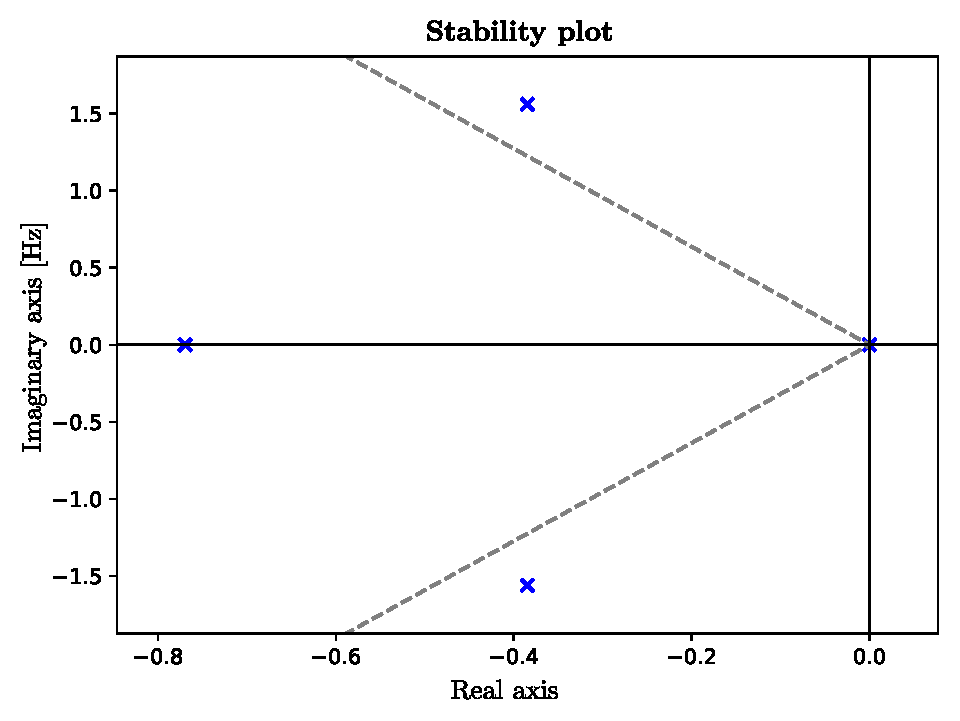
\includegraphics[width=0.8\linewidth]{inkscape_svg/eigenvalues_plot_example.pdf}
  \caption{Eigenvalue plot example.}
  \label{fig:eigenvalues_plot_example}
\end{figure}

The imaginary axis divide the stable part (negative real part) from the unstable part (positive real part). Therefore, all the eigenvalues
represented in the Figure are stable except for one which is in the origin, therefore the system is marginally stable. Moreover, modes outside
the real axis represent oscillatory modes. In this case, one can see that there are
two complex conjugate eigenvalues are represented, which means that the system has an oscillatory mode. the mode in the real axis is a non-oscillatory mode.
Since it is the one with the highest real part, it is the dominant mode of the system.



\subsection{Implementation}
The implementation of the small-signal stability analysis is divided mainly into two parts: the code development
 and the GUI implementation. 

\subsubsection{Code development}

The small-signal stability analysis is implemented in Python, following the general structure of the 
dynamic simulation framework in Veragrid. The general simulation structure for any simulation in VeraGrid
 is shown in Figure \ref{fig:General_Simulation_Structure}. 

\begin{figure}[H]
  \centering
  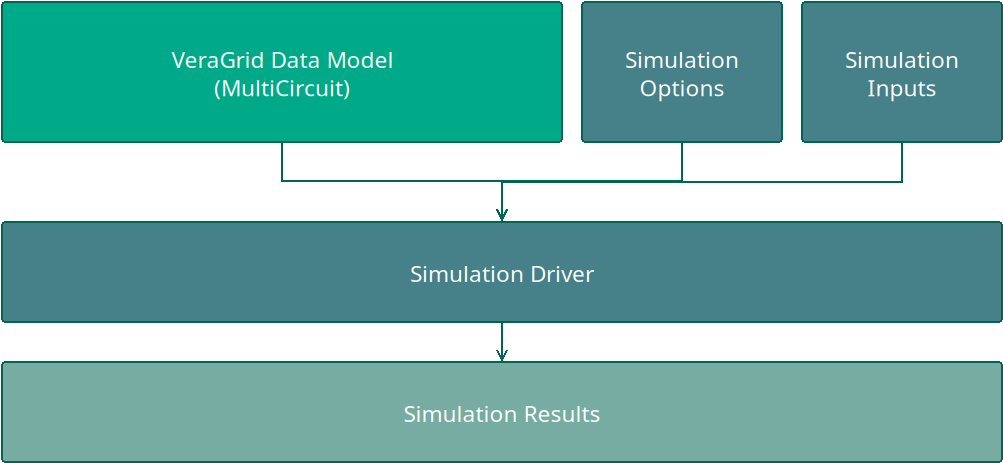
\includegraphics[width=0.8\linewidth]{figures/DataModelSimulationStructure.png}
  \caption{General simulation structure. \textit{Source: VeraGrid documentation \cite{veragrid}}}
  \label{fig:General_Simulation_Structure}
\end{figure}

Therefore, each simulation has three main classes explained below:

\begin{itemize}
    \item \textbf{Driver:} This class is responsible for running the simulation. It contains the simulation analysis function itself
    that computes the results and the run function that is called from the GUI, and it is responsible for executing the simulation.

    The block diagram of the small-signal stability analysis simulation function is shown in Figure \ref{fig:block_diagram_run_smallsignal}. 
    It consists on the A matrix computation from the jacobian matrix, the eigenvalues computation and then 2 main postprocesses: the participation factors
    computation and the damping ratios and oscillation frequencies computation. 
    
    The full simulation block diagram is shown in Figure \ref{fig:block_diagram_full_smallsignal} where one can see the main steps of the simulation from 
    importing the system data to the final results. The approach given is to give the user the option to run the small-signal stability analysis
    whenever he/she wants in the dynamic simulation. The user can initialize the system, check the stability in the first operation point, add an event and
    then check the stability again in the new operation point just choosing the assessment time.

    \item \textbf{Results:} This class is responsible for storing the results of the simulation. It contains the data structure that holds the results
    and the way they are accessed from the GUI. In this case, the results class show three main results: the eigenvalues with their corresponding damping ratios
    and oscillation frequencies, the participation factors matrix with the corresponding eigenvalues and states for each column and row respectively,
    and the complex plane plot of the eigenvalues in bot $rad/s$ and $Hz$ for the imaginary axis.

    \item \textbf{Options:} This class is responsible for defining the options of the simulation. It contains the parameters that can be set by the user
    from the GUI. In this case, the options class allows the user to set the assessment time, and in case the dynamic simulation is needed,
     the options for the simulation: integration method, time step and tolerance.
    
\end{itemize}

\begin{figure}[h]
  \centering
  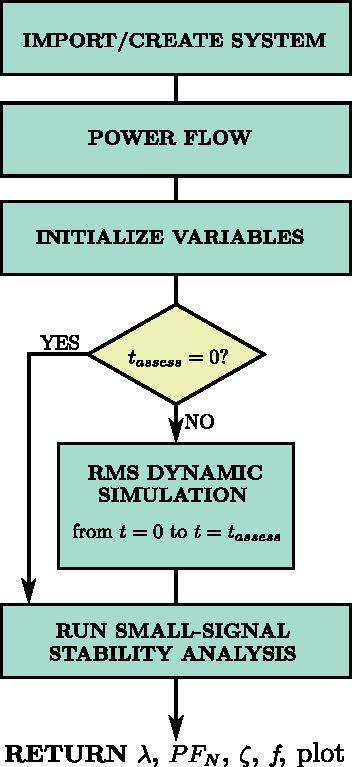
\includegraphics[width=0.35\linewidth]{inkscape_svg/block_diagram_full_code_smallsignal.pdf}
  \caption{Small-signal stability analysis full simulation block diagram. \textit{Source: Own elaboration.}}
  \label{fig:block_diagram_full_smallsignal}
\end{figure}

\begin{figure}[H]
  \centering
  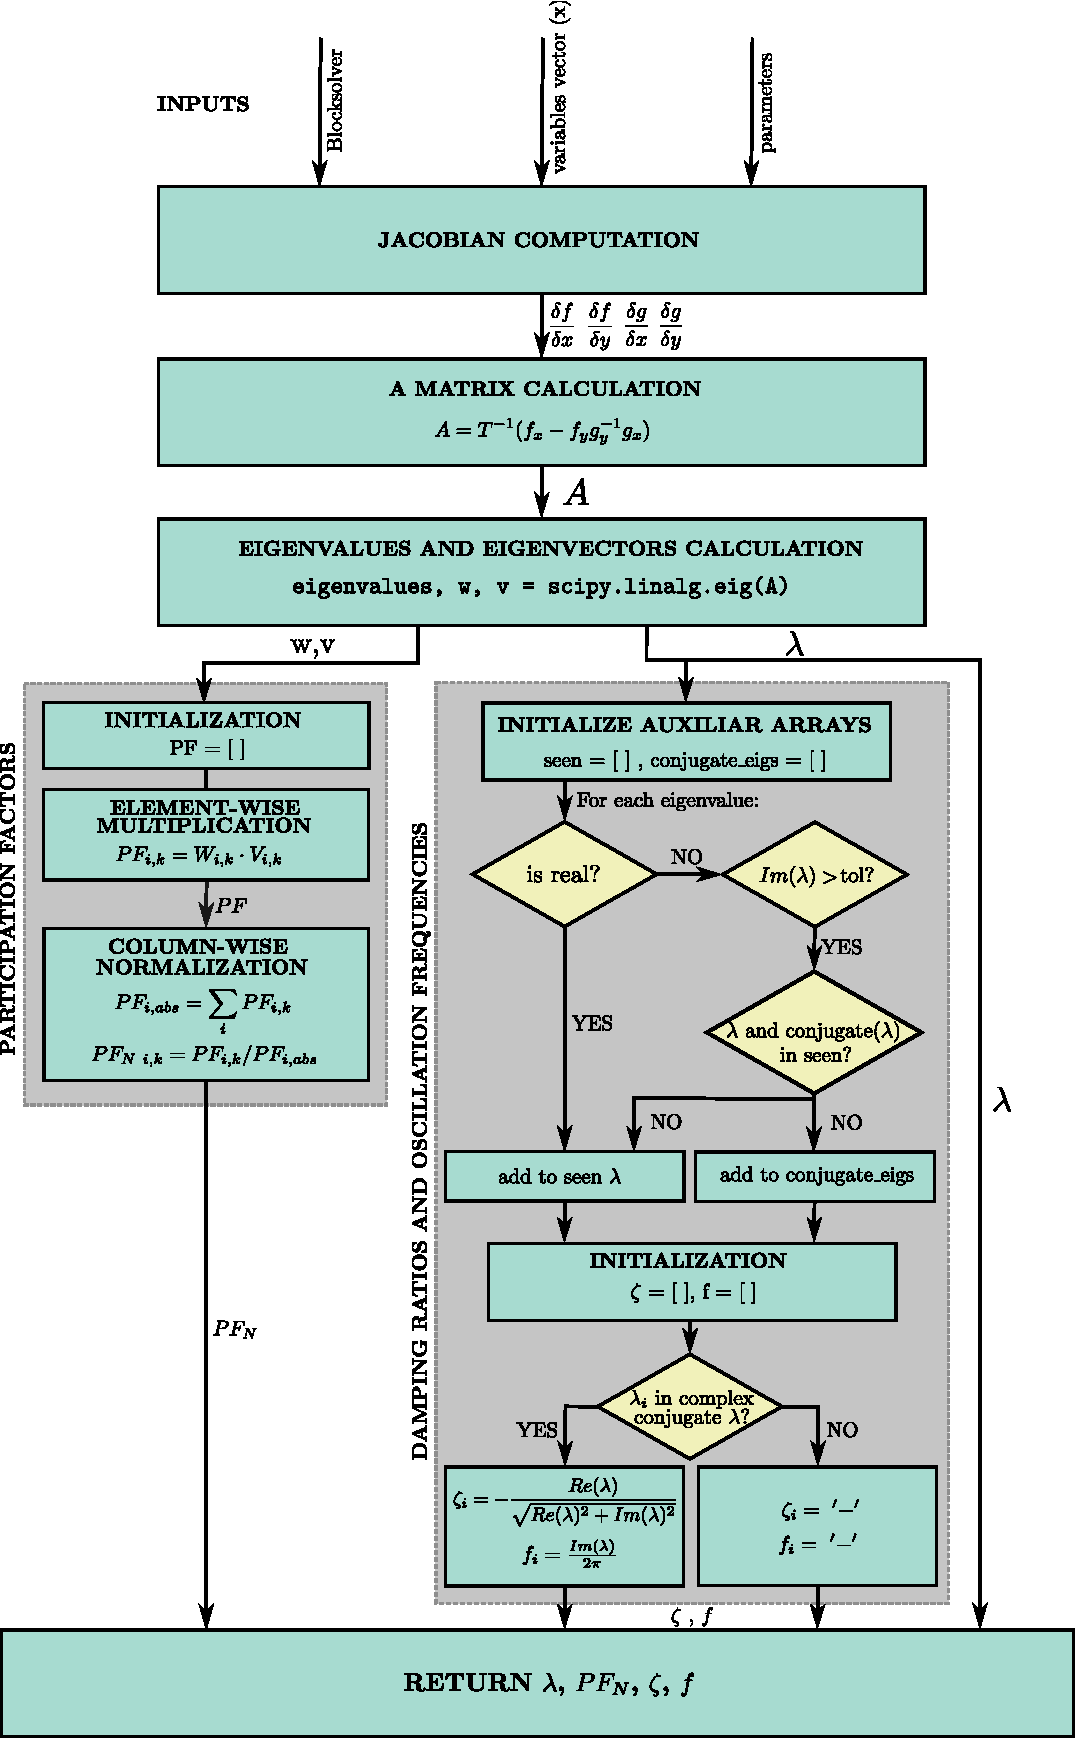
\includegraphics[width=0.8\linewidth]{inkscape_svg/block_diagram_run_smallsignal.pdf}
  \caption{Small-signal stability analysis computation block diagram. \textit{Source: Own elaboration.}}
  \label{fig:block_diagram_run_smallsignal}
\end{figure}

\subsubsection{GUI implementation}

The GUI is creased using the open source program Qt Designer \cite{qt_designer}, which allows to create the GUI using a drag 
and drop interface. The GUI implementation consists on creating a new settings page for the small-signal stability analysis,
adding the option to run the simulation in the main tools bar, and creating a new results page to show the results of the simulation. 
The GUI implementationis not only adding the new pages, but also connecting the GUI with the code developed in Python.

However, the first initial step is to choose an icon for the small-signal stability analysis that will be shown in the tools bar and will 
hels users identify the option. The icon chosen is shown in Figure \ref{fig:small_signal_icon}. The icon represents a magnifying glass 
looking at a wave. The magnifying glass represents the small-signal analysis, which works around a small perturbation and a small interval
around the operating point, so the user needs the magnifying glass to see those small perturbations. The wave represents the system variables
represented in the time domain, which are the ones that will be analysed in the small-signal stability analysis.

\begin{figure}[H]
  \centering
  
\includegraphics[width=0.25\linewidth]{inkscape_svg/small_signal_icon.pdf}
  \caption{Icon for the small-signal stability analysis. \textit{Source: VeraGrid \cite{veragrid}.}}
  \label{fig:small_signal_icon}
\end{figure}

The settings page shown in Figure \ref{fig:smallsignal_settings_GUI} allows the user to set the parameters needed for the small-signal stability analysis.
It is noted how the small-signal settings are added into the dynamic simulation settings. The settings shown are explained in the list below.

\begin{enumerate}
  \item \textit{Integration method}: The integration method to use if the RMS dynamic simulation is performed. There are two options: trapezoidal or implicit euler.
  \item \textit{Tolerance}: per-unit error tolerance to use in the integration method. Only needed if the Rms dynamic simulation is performed.
  \item \textit{Assessment time (s)}: The time instant in seconds where the stability assessment is performed.
  \item \textit{Time step (s)}: Step size in seconds between each numerical evaluation in the integration method. 
  Smaller intervals increase accuracy but require more computation. Only needed if the RMS dynamic simulation is performed.
\end{enumerate}


\begin{figure}[H]
  \centering
  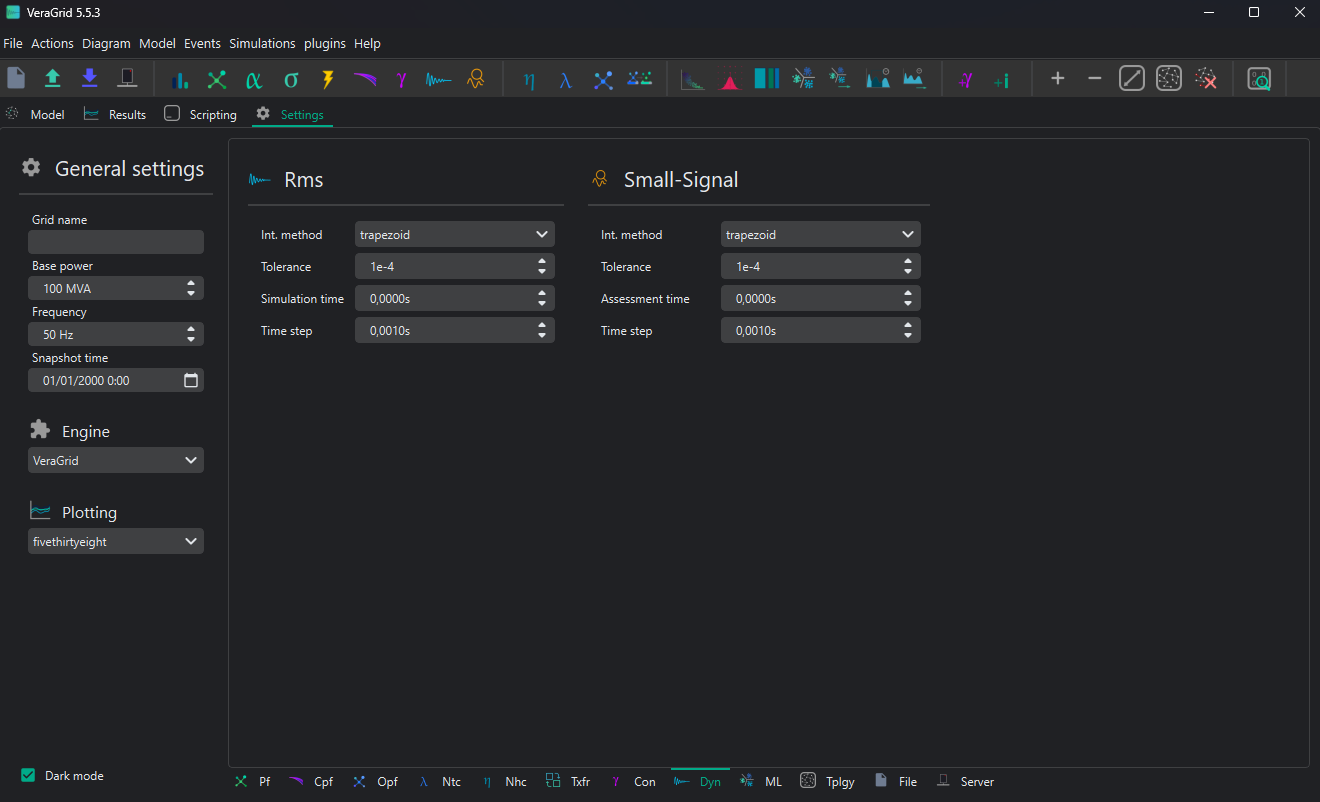
\includegraphics[width=0.8\linewidth]{figures/settings_GUI.png}
  \caption{Small-signal stability analysis settings page. \textit{Source: VeraGrid \cite{veragrid}.}}
  \label{fig:smallsignal_settings_GUI}
\end{figure}

Figure \ref{fig:model_powerflow_GUI} shows the model page with the power flow already computed. The small-signal stability analysis can 
only be performed if the power flow has been computed, as it is needed to obtain the operating point of the system.

\begin{figure}[H]
  \centering
  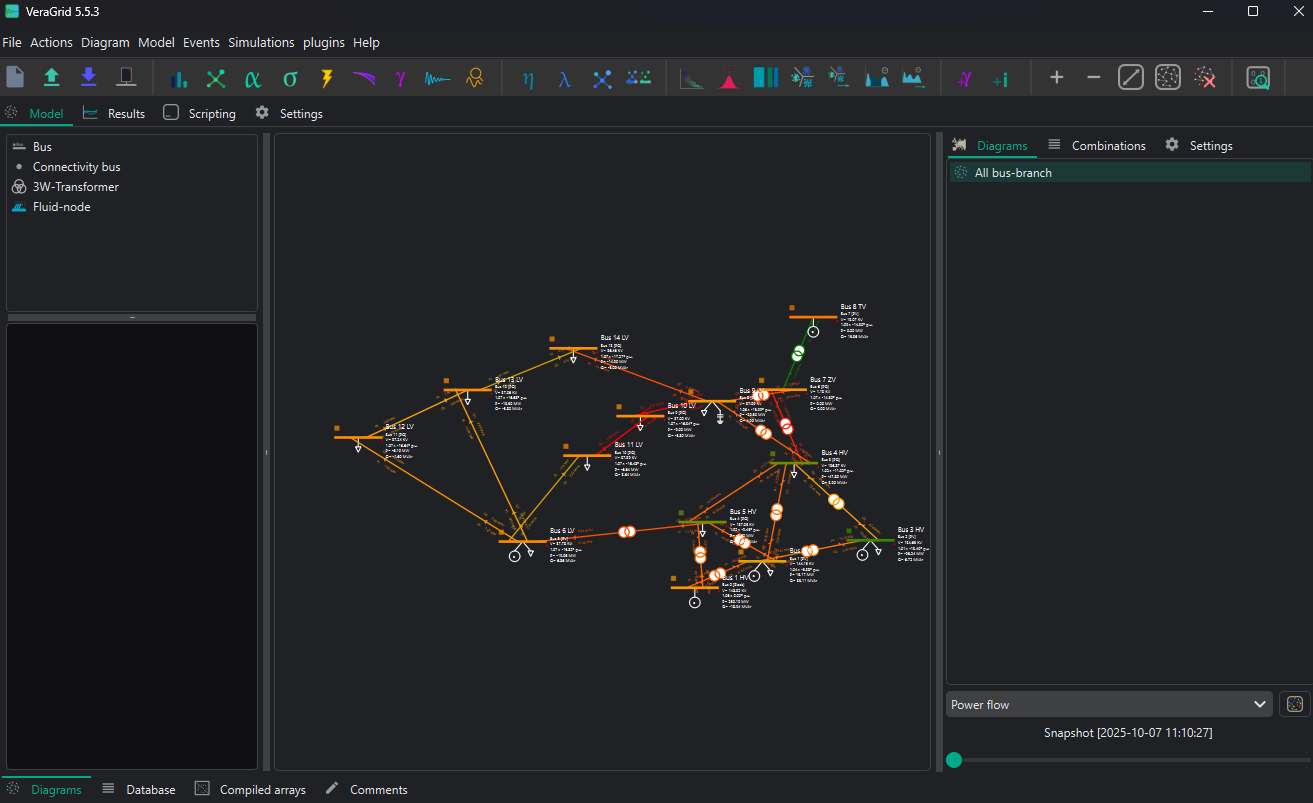
\includegraphics[width=0.8\linewidth]{figures/model_powerflow_GUI.png}
  \caption{Model page with power flow already computed. \textit{Source: VeraGrid \cite{veragrid}.}}
  \label{fig:model_powerflow_GUI}
\end{figure}

\begin{figure}[H]
  \centering
  \begin{minipage}{0.45\textwidth}
    \centering
    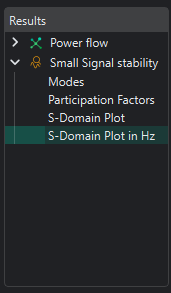
\includegraphics[width=0.5\linewidth]{figures/results_desplegable_GUI.png}
    \caption{Results drowdown. \textit{Source: VeraGrid \cite{veragrid}.}}
    \label{fig:results_dropdown_GUI}
  \end{minipage}
  \hfill
  \begin{minipage}{0.5\textwidth}
    The results page shows the results of all the simulations performed in VeraGrid. The user can choose the results to show
    using the dropdown menu shown in Figure \ref{fig:results_dropdown_GUI}. In this case, the power flow and small-signal stability
     analysis results are shown. As one can see, the small-signal results are divided into 4 options: the modes table, the participation
     factors table, the complex domain plot and the complex domain plot in Hz. These results are shown in Figures \ref{fig:table_modes_GUI},
     \ref{fig:table_PF_GUI}, \ref{fig:plot_ss_GUI} and \ref{fig:plot_ss_Hz_GUI} respectively.
  \end{minipage}
\end{figure}

\begin{figure}[H]
  \centering
  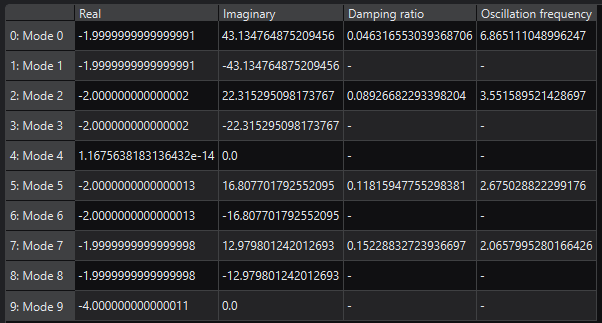
\includegraphics[width=0.8\linewidth]{figures/result_modes_ss_GUI.png}
  \caption{Table result with the modes, damping ratio and oscillation frequencies. \textit{Source: VeraGrid \cite{veragrid}.}}
  \label{fig:table_modes_GUI}
\end{figure}

\begin{figure}[H]
  \centering
  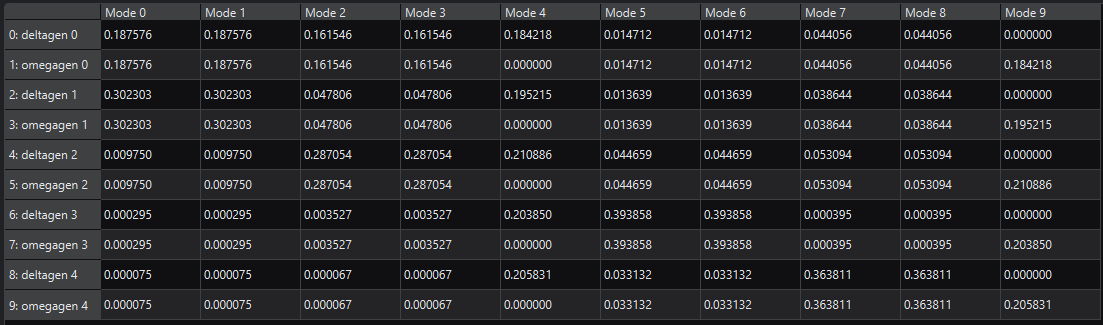
\includegraphics[width=1\linewidth]{figures/result_pfactors_GUI.png}
  \caption{Table result with the participation factors. \textit{Source: VeraGrid \cite{veragrid}.}}
  \label{fig:table_PF_GUI}
\end{figure}

\begin{figure}[H]
  \centering
  \begin{minipage}{0.49\textwidth}
    \centering
    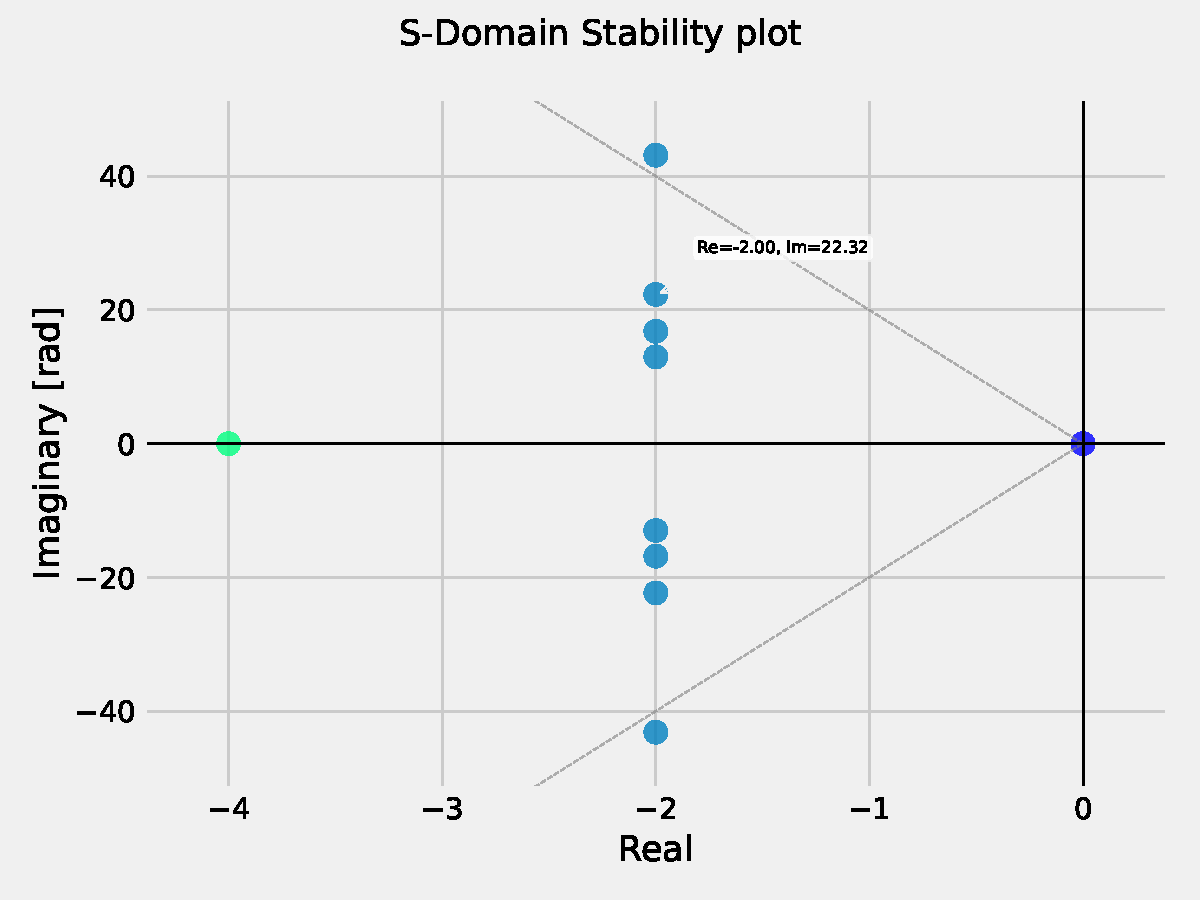
\includegraphics[width=\linewidth]{figures/smallsignal_plot_GUI.pdf}
    \caption{Complex domain plot.  \textit{Source: VeraGrid \cite{veragrid}.}}
    \label{fig:plot_ss_GUI}
  \end{minipage}
  \hfill
  \begin{minipage}{0.49\textwidth}
    \centering
    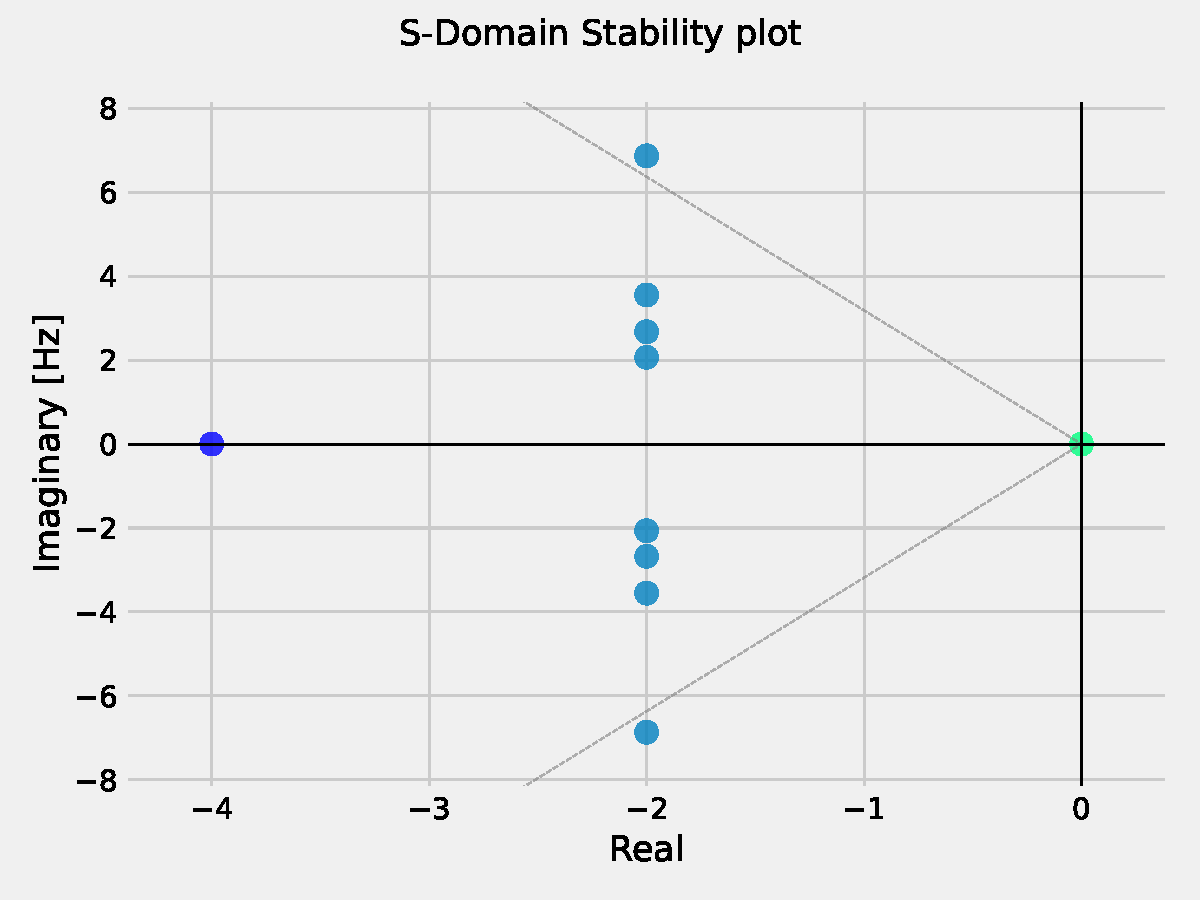
\includegraphics[width=\linewidth]{figures/smallsignal_plot_Hz_GUI.pdf}
    \caption{Complex domain plot in Hz. \textit{Source: VeraGrid \cite{veragrid}.}}
    \label{fig:plot_ss_Hz_GUI}
  \end{minipage}
\end{figure}

Figure \ref{fig:plot_ss_GUI} shows how the user can take a look at the eigenvalues exact values
by hovering the mouse over the points. Moreover, the 5\% damping ratio line is shown to help the user identify
the unstable modes. 









\subsection{Benchmark and validation}
%BENCHMARK SMALL-SIGNAL STABILITY ANALYSIS

The validation of the developed implementation is performed by comparing its results with those obtained using 
\textit{Advanced Network Dynamics and Equilibrium Simulator} (ANDES). The comparison is carried out on the classical Kundur two-area test system, 
a standard benchmark for dynamic systems, enabling a direct verification the small-signal stability analysis between both tools.


\subsubsection{ANDES}

Thanks to its combination of symbolic precision and robust numerical performance, \textit{Advanced Network Dynamics and Equilibrium Simulator} (ANDES) 
provides an excellent reference platform for the validation of dynamic and stability analysis tools in modern power system research. 
Developed as an open-source framework for modelling differential-algebraic systems, ANDES enables a fully symbolic formulation of network equations and 
control models, which ensures reproducibility and analytical transparency across a wide range of test systems. 
For these reasons, ANDES is widely recognised as a reliable benchmark for many types of simulations such as small-signal stability studies and has been 
used here as the reference software against which the performance of VeraGrid has been assessed.

\begin{figure}[H]
    \centering
    
\includegraphics[width=0.9\linewidth]{figures/ANDES_banner.png}
    \caption{ANDES logo. \textit{Source}: ANDES documentation \cite{andes}.}
\end{figure}

VeraGrid imports ANDES models directly from standardized \texttt{.json} files, allowing the seamless translation of system data, dynamic models, 
and numerical parameters. Once imported, VeraGrid performs the ANDES small-signal stability computations internally, based on ANDES numerical engine. 
The results obtained from VeraGrid have been compared with those from ANDES. VeraGrid successfully reproduces the full set of eigenvalues,
damping ratios, and oscillation frequencies computed by ANDES, confirming the equivalence of its linearisation procedures and numerical solvers. 

Beyond direct eigenvalue matching, the validation process also includes the comparison of mode shapes, damping factors, and participation factors
matrices to ensure consistency in both the algebraic formulation and numerical sensitivity of the two tools. These extended checks are essential to 
confirm that the dynamic responses, not only the eigenvalue, coincide under identical modelling assumptions. In practice, this guarantees that VeraGrid 
preserves the physical interpretation of oscillatory modes and stability margins originally provided by ANDES, while operating within its own software framework.

In the following subsection the Kundur two-area system is used as a benchmark test case to illustrate the accuracy of VeraGrid in reproducing ANDES results.


\subsubsection{Test case: Kundur two-area system}

The Kundur two-area system is a standard benchmark network widely used for small-signal and transient stability studies.
 It was introduced in the P. Kundur power system stability literature \cite{StabilityAndControlKundur} as a compact, yet representative, test case that exposes 
 inter-area oscillatory modes and control interactions without excessive model complexity.

\begin{figure}[h!]
    \centering
    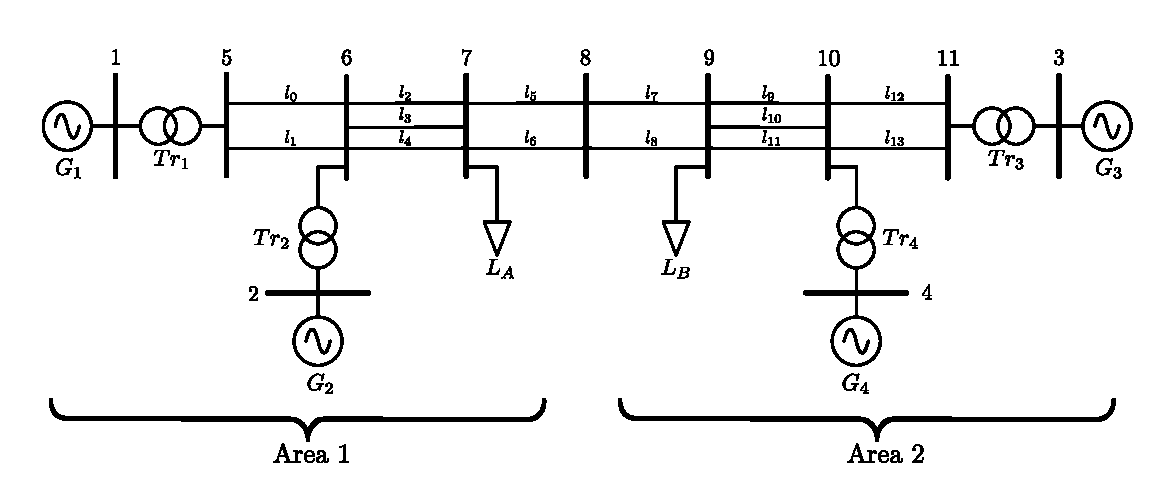
\includegraphics[width=1\linewidth]{inkscape_svg/Kundur_system_no_shunt.pdf}
    \caption{Kundur two-area system without shunt.}
    \label{fig:kundur_system}
\end{figure}

Figure \ref{fig:kundur_system} shows the one-line diagram of the Kundur two-area system without shunt. The main characteristics of the system are the following:
\begin{itemize}
    \item There are two areas connected by a pair of parallel lines. In each area, 2 synchronous generators are placed so that each area can swing against 
    each other and produce inter-area oscillations.
    \item All the synchronous generators are connected to the network through a transformer.
    \item In this version of the Kundur two-area system no shunts are connected to buses 7 and 9.
    \item While the system seems exactly symmetrical, the loads and generators are not exactly equal. This provoques the need of power exchange between areas.
\end{itemize}

Table \ref{tab:properties_kundur} summarizes the parameters of the system.

\begin{table}[H]
\centering
\caption{Main parameters of the Kundur two-area system without shunts.}
\label{tab:properties_kundur}
\renewcommand{\arraystretch}{1.2}
\small
\begin{tabular}{|l|l|l|l|}
\hline
\textbf{Element} & \textbf{Parameter} & \textbf{Symbol / Value} & \textbf{Units / Notes} \\ 
\hline

\multicolumn{4}{|l|}{\textbf{Buses}} \\ 
\hline
Bus1 to 4 & Nominal voltage & $20$ & kV \\ 
Bus5 to 11 & Nominal voltage & $230$ & kV \\ 
\hline

\multicolumn{4}{|l|}{\textbf{Generators}} \\ 
\hline
G1, G2 & Nominal Power & $900$ & MVA \\ 
       & Nominal voltage & $20$ & kV \\ 
       & Inertia constant & $M = 13$ & s \\ 
       & Damping coefficient & $D = 10$ & -- \\ 
       & Impedances & $r_a = 0,0$, $x_d = 0,3$ & p.u. \\ 
G3, G4 & Nominal Power & $900$ & MVA \\ 
       & Nominal voltage & $20$ & kV \\ 
       & Inertia constant & $M = 12,35$ & s \\ 
       & Damping coefficient & $D = 10$ & -- \\ 
       & Impedances & $r_a = 0,0$, $x_d = 0,3$ & p.u. \\ 
\hline

\multicolumn{4}{|l|}{\textbf{Transformers}} \\ 
\hline
Tr 1, 2, 3, 4 & Impedance & $R = 0,0$, $X = 0,15$, $B = 0,0$ & p.u. \\ 
               & Rate & $900$ & MVA \\ 
\hline

\multicolumn{4}{|l|}{\textbf{Transmission lines}} \\ 
\hline
Line 0, 1, 12, 13 & Impedance & $R = 0,005$, $X = 0,05$, $B = 0,02187$ & p.u. \\ 
                   & Rate & $750$ & MVA \\ 
Line 2, 3, 4, 9, 10, 11 & Impedance & $R = 0,003$, $X = 0,03$, $B = 0,00583$ & p.u. \\ 
                         & Rate & $700$ & MVA \\ 
Line 5, 6, 7, 8 (tie-line) & Impedance & $R = 0,011$, $X = 0,11$, $B = 0,19250$ & p.u. \\ 
                            & Rate & $400$ & MVA \\ 
\hline
\multicolumn{4}{|l|}{\textbf{Loads}} \\ 
\hline
Load A & Power & $P_L = 967$, $Q_L = 100$ & MW, Mvar \\ 
Load B & Power & $P_L = 1767$, $Q_L = 100$ & MW, Mvar \\ 
\hline

\end{tabular}
\end{table}

\begin{figure}[H]
  \centering
  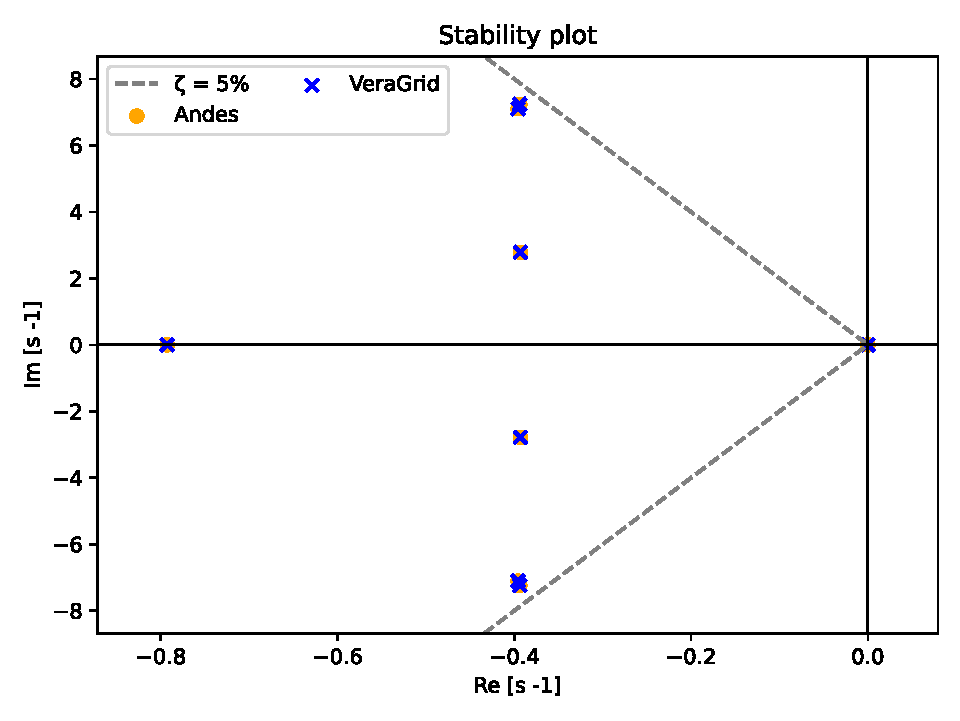
\includegraphics[width=0.7\linewidth]{inkscape_svg/andes_vs_veragrid_kundur.pdf}
  \caption{Andes vs VeraGrid complex domain plot comparison.}
  \label{fig:AndesvsVeraGrid}
\end{figure}


Figure \ref{fig:AndesvsVeraGrid} shows the comparison in the complex plane of the eigenvalues obtained
with VeraGrid and Andes for the Kundur two-area system without shunts, while Tables \ref{tab:eigenvalues_kundur} and
\ref{tab:pfactors_kundur} show the modes, damping ratios, oscillation frequencies and participation factors of the system.
The results between Andes and VeraGrid are practically identical, 
with less than 0,0001\% absolute error, this one due to numerical computation differences.


\begin{table}[H]
\centering
\caption{Modes, damping ratios and oscillation frequencies of the Kundur Two-Area System.}
\label{tab:eigenvalues_kundur}
\renewcommand{\arraystretch}{1.2}
\small
\begin{tabular}{|c|c|c|c|c|}
\hline
\textbf{Mode} & \textbf{Real part} & \textbf{Imaginary part} & \textbf{Damping ratio} & \textbf{Oscillation Frequency [Hz]} \\ 
\hline
Mode 0 & -0,3938 & 7,2377 & 0,0543 & 1,1519 \\
Mode 1 & -0,3938 & -7,2377 & -- & -- \\
Mode 2 & -0,3958 & 7,1061 & 0,0556 & 1,1310 \\
Mode 3 & -0,3958 & -7,1061 & -- & -- \\
Mode 4 & -0,3931 & 2,7838 & 0,1398 & 0,4431 \\
Mode 5 & -0,3931 & -2,7838 & -- & -- \\
Mode 6 & 0,0000  & 0,0000  & -- & -- \\
Mode 7 & -0,7926 & 0,0000  & -- & -- \\
\hline
\end{tabular}
\end{table}


\begin{table}[H]
\centering
\caption{Participation factors of the Kundur two-area system.}
\label{tab:pfactors_kundur}
\renewcommand{\arraystretch}{1.2}
\small
\begin{tabular}{|c|cccccccc|}
\hline
\textbf{State/Mode} & \textbf{Mode 0} & \textbf{Mode 1} & \textbf{Mode 2} & \textbf{Mode 3} & \textbf{Mode 4} & \textbf{Mode 5} & \textbf{Mode 6} & \textbf{Mode 7} \\ 
\hline
$\delta_1$ & 0,123 & 0,123 & 0,102 & 0,102 & 0,174 & 0,174 & 0,197 & 0,006 \\
$\omega_1$ & 0,123 & 0,123 & 0,102 & 0,102 & 0,174 & 0,174 & 0,000 & 0,197 \\
$\delta_2$ & 0,151 & 0,151 & 0,122 & 0,122 & 0,117 & 0,117 & 0,214 & 0,006 \\
$\omega_2$ & 0,151 & 0,151 & 0,122 & 0,122 & 0,117 & 0,117 & 0,000 & 0,214 \\
$\delta_3$ & 0,103 & 0,103 & 0,157 & 0,157 & 0,102 & 0,102 & 0,283 & 0,006 \\
$\omega_3$ & 0,103 & 0,103 & 0,156 & 0,156 & 0,102 & 0,102 & 0,000 & 0,272 \\
$\delta_4$ & 0,123 & 0,123 & 0,119 & 0,119 & 0,108 & 0,108 & 0,306 & 0,006 \\
$\omega_4$ & 0,123 & 0,123 & 0,119 & 0,119 & 0,107 & 0,107 & 0,000 & 0,293 \\
\hline
\end{tabular}
\end{table}



The small-signal stability analysis of the Kundur two-area system shows that the system is asymptotically stable, 
despite the presence of one zero eigenvalue associated with the rigid-body motion. Three oscillatory
mode pairs are identified: two local modes around 1,14~Hz with damping ratios of about 5,5\%, 
and one inter-area mode at 0,44~Hz with a damping ratio of 13,98\%. In addition, two real modes appear,
the dominant pole -0,7962 corresponding to a fast mechanical decay and another representing the neutral 
reference frame.

The local modes are associated with oscillations of the generators within the same area against one another. 
In this case, two pairs of complex conjugate eigenvalues located at $-0,3938 \pm j7,2377$ and $-0,3958 \pm j7,1061$ correspond to frequencies
 of $1,1519$ and $1,1310$~Hz respectively with damping ratios near $5,5\%$. These modes involve mainly the rotor angles and 
 speeds of generators within each area, indicating local electromechanical interactions between closely coupled machines. The higher frequencies reflect the local nature of these oscillations, which are typically faster than inter-area modes due to the stronger electrical coupling and lower inertia involved. 
 The relatively low damping (just above the threshold 5\%) means that oscillations at these frequencies would decay slowly after a 
 disturbance, and therefore these modes are usually targeted for improvement through power system stabilizers designed to increase 
 the effective damping while maintaining the natural frequency range around one hertz.

The inter-area mode, represented by the eigenvalue pair $-0,3931 \pm j2,7838$, exhibits a frequency of  $0,4431$~Hz and a damping 
ratio of $13,98\%$. The participation factors show that the mode involves the collective motion of generators in one area oscillating 
against those in the other, with all machines in each group moving coherently. This behavior reflects the exchange of power 
through the tie-line connecting the two subsystems, which gives rise to slow, large-scale oscillations of the inter-area type. 
The relatively higher damping compared with the local modes suggests that the tie-line 
contribute sufficient stabilizing torque under the present operating point. Nevertheless, variations in power transfer or network 
strength could reduce this damping and make the inter-area oscillation more critical, as observed in many large interconnected grids.

Among the real modes, one negative mode at approximately $-0,7926$ represents a non-oscillatory but fast-decaying mode, 
mainly related to the mechanical dynamics of the generating units. Its time constant ($\tau = -1/Re(\lambda)$), around $1,26$~s, indicates a rapid stabilizing
effect that brings the system back to equilibrium after active-power mismatches or primary control actions. This mode is considered 
dominant in the sense that it governs the short-term return to balance but does not limit the overall stability margins of the system.

Finally, the eigenvalue located at the origin, $\lambda = 0$, corresponds to the uniform or rigid-body mode. 
Mathematically, it indicates marginal stability, as perturbations projected onto this mode neither grow nor decay.
Physically, however, it simply reflects the absence of an absolute angular reference: if all generator rotor angles are shifted by the same constant, 
the electrical state of the system remains unchanged. Only differences in rotor angles carry physical meaning, so this mode has no effect on the stability 
of the relative motion among machines. In practical studies, this degree of freedom is not considered for the stability analysis. 
Consequently, although the rigid-body mode is formally marginally stable, it is not regarded as a sign of instability in the power system.
 
These results are consistent with the classical interpretation of the two-area system and confirm its suitability as a benchmark
 for dynamic studies.




\newpage

\section{EMT Dynamic framework}\label{Chap2}


\newpage

\section{Environmental, Social, and Gender Impact}

\section{Environmental impact}

An environmental contribution of this work lies in its support for energy efficiency and the 
ongoing energy transition. The developed framework contributes to the optimal operation and planning
of power systems with high shares of renewable generation. Stability analysis allows network operators to 
safely integrate variable renewable sources such as wind and solar while maintaining system reliability. 
This, in turn, facilitates higher utilization of clean energy resources and reduces curtailment, 
leading to a more efficient use of installed capacity and a measurable reduction in carbon emissions. 
In a broader context, the development of robust and open simulation tools is essential to achieving global 
decarbonisation objectives and ensuring a stable, sustainable transition towards a low-carbon energy system \cite{IEA2024Transition}.

Although the present work involves primarily computational and simulation tasks rather than physical infrastructure,
it nonetheless carries meaningful environmental implications. Advanced RMS and EMT tools aid in the integration of 
renewable energy sources by improving the predictability and security of grid behavior, thereby helping reduce
reliance on fossil fuel backup plants and associated greenhouse gas emissions\cite{XiongParaEMT2024}. 
The trade-off between simulation fidelity and computational cost is also well documented; for example, Yan et al.\ examine
the impact of different numerical integration schemes on simulation accuracy and efficiency \cite{YanCompEff2025}. 
Minimizing computational energy consumption through algorithmic optimization is thus a relevant concern.

Moreover, the promotion of open-source platforms in power system research enhances resource efficiency by reducing 
duplicated development efforts and enabling community-driven innovation. The use of openly shared modeling libraries 
accelerates progress and lowers barriers to entry\cite{TesfatsionOpenSource}. By providing validated simulation tools, 
this work contributes to more sustainable and cost-effective grid planning, potentially reducing the environmental 
footprint of energy infrastructure expansion.

On the other side, the actual footprint of the project development can be computed as kg of $CO_2$ equivalent emitted
to the atmosphere. This study estimates the direct environmental footprint accounting for the
electricity consumed by the computer and monitor, the corresponding share of HVAC energy use and the amortized embodied 
emissions of the electronic equipment. 
The calculation considers a five-month period (September to January), with a working schedule of eight hours per day, Monday to Friday. 
This corresponds to approximately $22$~weeks~$ \cdot $~5~days/week~$ \cdot $~8~h/day~$\approx~880$~hours.

The working environment corresponds to a small office space in the center of Barcelona, shared by approximately 20 occupants. In order to simplify the 
study, the following assumptions are done:

\begin{itemize}
    \item Only the energy used by the laptop and the monitor are considered.
    \item The kg of $CO_2$ equivalent emitted by the manufacturing and transportation of the laptop and monitor are considered. The office equipment is not considered.
    \item Only the energy consumption due to HVAC in the office is considered due to its high contribution to energy consumption in the office.
\end{itemize}


For the Laptop embodied emissions Circular Computing \cite{CircularComputing2022} proposes 331~kg\,CO$_2$eq/device accounting for manufacturing,
transport and 4 first years of use. According to their calculations, manufacturing and transport accounts by approximately 90\% of those emissions.
For the monitor, a standard monitor has been selected. HP sustainability report \cite{HP2021MonitorLCA} states that 210~kg\,CO$_2$eq/device 
are emitted during manufacturing, transport, use and end of life. Manufacturing, transport and end of life account for a 47\% of those emissions.
According to l'Institut Català de l'Energia (ICAEN) \cite{ICAEN}, the recommended average HVAC energy consumption in an office building is 140~kWh/m$^2$~year. 
Scaling this consumption to an average of 5m$^2$ per person in a office and 260 working days a year the resulting energy consumption is 
0,299 kWh/hour~person. For the allocation factor of the laptop and monitor, 5 years of lifespan are assumed.

All parameters used are summarized in Table~\ref{tab:co2_inputs_full}.

\begin{table}[H]
\centering
\caption{Emission factors and embodied carbon data used in the estimation.}
\label{tab:co2_inputs_full}
\renewcommand{\arraystretch}{1.15}
\small
\begin{tabular}{|l|c|c|l|}
\hline
\textbf{Source / Component} & \textbf{Value} & \textbf{Unit} & \textbf{Reference} \\ 
\hline
Electricity emission factor (Spain, 2023) & 0,26 & kg\,CO$_2$eq/kWh & \cite{Gencat2023FactorsEmissio} \\ 
Laptop embodied emissions (manufacturing) & 297,9 & kg\,CO$_2$eq/device & \cite{CircularComputing2022} \\ 
Monitor embodied emissions (manufacturing) & 94,47 & kg\,CO$_2$eq/device & \cite{HP2021MonitorLCA} \\ 
Average laptop power draw & 45 & W & \cite{AsusVivabook} \\ 
Average monitor power draw & 37 & W & \cite{AOC} \\ 
HVAC energy use per occupant (shared office) & 0,299 & kWh/h~pers & \cite{ICAEN} \\ 
Allocation factor laptop and monitor & 0.084 & -- & assumed \\ 
\hline
\end{tabular}
\end{table}

The total electricity consumption during the five-month period can be expressed as:

\begin{equation}
E_{total} = E_{PC+monitor}  + E_{HVAC}~[kWh]
\end{equation}
where:

\begin{equation}
E_{PC+monitor} = (P_L~W + P_M ~W) \cdot  \frac{880~h}{1000~W/kW} = 72,16 kWh
\end{equation}
\begin{equation}
E_{HVAC} = 0,299~kWh/h \cdot 880~h = 263,25~kWh
\end{equation}

Corresponding to a total of 87,206 kg of CO$_2$eq due to energy consumption.

The allocation contribution of the LCA for the laptop and monitor correspond to a total of $(297,9 + 94,47)$~kg~CO$_2$eq $\cdot 0,084 = 32,959$~kg~CO$_2$eq.

The total emissions are 120,165 kg of CO$_2$eq. Table \ref{tab:contribution_CO2} summarizes the contribution of each element to the total 

\begin{table}[H]
\centering
\caption{Estimated carbon footprint of the thesis work including HVAC, lighting, and office equipment.}
\label{tab:contribution_CO2}
\renewcommand{\arraystretch}{1.15}
\small
\begin{tabular}{|l|c|c|}
\hline
\textbf{Component} & \textbf{kg\,CO$_2$eq emissions } & \textbf{Contribution} \\ 
\hline
Laptop + monitor operation & $18,761$ & $15,613~\%$ \\ 
HVAC energy consumption & $68,444$ & $56,958~\%$ \\ 
Allocated embodied emissions (laptop + monitor) & $32,959$ & $27,428~\%$ \\ 
\hline
\textbf{Total estimated footprint} & \textbf{120,165} &  \\ 
\hline
\end{tabular}
\end{table}

Results conclude that the main contribution to the project development global emissions are due to the office HVAC being the 56,95\% of 
the total equivalent CO$_2$ emissions. Regarding the laptop and monitor it is seen how the manufacturing and transporting contribution
is much higher than the operation itself, highlighting the importance of Life Cycle Assessments on the environmental assessments.

To contextualize the estimated footprint of this work, it is useful to compare it with reference studies on greenhouse gas emissions in office environments. 
According to the European Environment Agency, the annual emissions associated with a standard office workplace in 
Europe (including HVAC, lighting, equipment, and commuting) are between 1500 and 2000~kg\,CO$_2$eq per employee \cite{EEA2021OfficeEnergy}. The corresponding contribution
of 5 months is  between 625 and 833~kg\,CO$_2$eq. As noted, in this study the EEA considers also the commuting to work. Circular Ecology \cite{CircularEcology} states that, in Europe. only 53\%
of the emissions of going to work in an office account for the office itself meaning 47\% of the emissions correspond to commuting. Applying this percentage
the average office emissions(including HVAC, lighting, equipment) in Europe are between 331,250 and 441,677~kg\,CO$_2$eq.

In comparison, the total estimated footprint of approximately 120~kg\,CO$_2$eq for this thesis project is lower than the studies stated in the previous paragraph.
It is to be considered that the EEA study considers both lightning and equipment while this study does not. Moreover, the average energy consumption in Europe is
higher than in Spain so this result may be affected. Therefore, the result is considered correct and highlights the importance of energy-efficient habits.

\section{Gender and social impact}

TO CHECK!!

Beyond technical contributions, this project supports broader social goals through the promotion of inclusive and accessible tools. 
Open-source frameworks for power system analysis democratize advanced engineering capabilities, enabling participation from researchers 
and engineers in diverse regions and institutions. For instance, the development of open and transparent electricity network 
models demonstrates how access to modeling tools can empower under-resourced communities \cite{KirliPyPSA2021}. Open-source frameworks
support the idea that knowledgment must be a social right and accessible for everybody.

From a gender perspective, power systems engineering remains dominated by men in many contexts. Disseminating open methodologies 
and encouraging diverse collaboration may help widen participation of underrepresented groups in STEM fields. 

Finally, improving the reliability, stability, and efficiency of power systems has direct social benefits: fewer outages, better access to electricity, 
and more resilient grids that support sustainable development goals.  



\newpage

\section{}

\section{Environmental impact}

An environmental contribution of this work lies in its support for energy efficiency and the 
ongoing energy transition. The developed framework contributes to the optimal operation and planning
of power systems with high shares of renewable generation. Stability analysis allows network operators to 
safely integrate variable renewable sources such as wind and solar while maintaining system reliability. 
This, in turn, facilitates higher utilization of clean energy resources and reduces curtailment, 
leading to a more efficient use of installed capacity and a measurable reduction in carbon emissions. 
In a broader context, the development of robust and open simulation tools is essential to achieving global 
decarbonisation objectives and ensuring a stable, sustainable transition towards a low-carbon energy system \cite{IEA2024Transition}.

Although the present work involves primarily computational and simulation tasks rather than physical infrastructure,
it nonetheless carries meaningful environmental implications. Advanced RMS and EMT tools aid in the integration of 
renewable energy sources by improving the predictability and security of grid behavior, thereby helping reduce
reliance on fossil fuel backup plants and associated greenhouse gas emissions\cite{XiongParaEMT2024}. 
The trade-off between simulation fidelity and computational cost is also well documented; for example, Yan et al.\ examine
the impact of different numerical integration schemes on simulation accuracy and efficiency \cite{YanCompEff2025}. 
Minimizing computational energy consumption through algorithmic optimization is thus a relevant concern.

Moreover, the promotion of open-source platforms in power system research enhances resource efficiency by reducing 
duplicated development efforts and enabling community-driven innovation. The use of openly shared modeling libraries 
accelerates progress and lowers barriers to entry\cite{TesfatsionOpenSource}. By providing validated simulation tools, 
this work contributes to more sustainable and cost-effective grid planning, potentially reducing the environmental 
footprint of energy infrastructure expansion.

On the other side, the actual footprint of the project development can be computed as kg of $CO_2$ equivalent emitted
to the atmosphere. This study estimates the direct environmental footprint accounting for the
electricity consumed by the computer and monitor, the corresponding share of HVAC energy use and the amortized embodied 
emissions of the electronic equipment. 
The calculation considers a five-month period (September to January), with a working schedule of eight hours per day, Monday to Friday. 
This corresponds to approximately $22$~weeks~$ \cdot $~5~days/week~$ \cdot $~8~h/day~$\approx~880$~hours.

The working environment corresponds to a small office space in the center of Barcelona, shared by approximately 20 occupants. In order to simplify the 
study, the following assumptions are done:

\begin{itemize}
    \item Only the energy used by the laptop and the monitor are considered.
    \item The kg of $CO_2$ equivalent emitted by the manufacturing and transportation of the laptop and monitor are considered. The office equipment is not considered.
    \item Only the energy consumption due to HVAC in the office is considered due to its high contribution to energy consumption in the office.
\end{itemize}


For the Laptop embodied emissions Circular Computing \cite{CircularComputing2022} proposes 331~kg\,CO$_2$eq/device accounting for manufacturing,
transport and 4 first years of use. According to their calculations, manufacturing and transport accounts by approximately 90\% of those emissions.
For the monitor, a standard monitor has been selected. HP sustainability report \cite{HP2021MonitorLCA} states that 210~kg\,CO$_2$eq/device 
are emitted during manufacturing, transport, use and end of life. Manufacturing, transport and end of life account for a 47\% of those emissions.
According to l'Institut Català de l'Energia (ICAEN) \cite{ICAEN}, the recommended average HVAC energy consumption in an office building is 140~kWh/m$^2$~year. 
Scaling this consumption to an average of 5m$^2$ per person in a office and 260 working days a year the resulting energy consumption is 
0,299 kWh/hour~person. For the allocation factor of the laptop and monitor, 5 years of lifespan are assumed.

All parameters used are summarized in Table~\ref{tab:co2_inputs_full}.

\begin{table}[H]
\centering
\caption{Emission factors and embodied carbon data used in the estimation.}
\label{tab:co2_inputs_full}
\renewcommand{\arraystretch}{1.15}
\small
\begin{tabular}{|l|c|c|l|}
\hline
\textbf{Source / Component} & \textbf{Value} & \textbf{Unit} & \textbf{Reference} \\ 
\hline
Electricity emission factor (Spain, 2023) & 0,26 & kg\,CO$_2$eq/kWh & \cite{Gencat2023FactorsEmissio} \\ 
Laptop embodied emissions (manufacturing) & 297,9 & kg\,CO$_2$eq/device & \cite{CircularComputing2022} \\ 
Monitor embodied emissions (manufacturing) & 94,47 & kg\,CO$_2$eq/device & \cite{HP2021MonitorLCA} \\ 
Average laptop power draw & 45 & W & \cite{AsusVivabook} \\ 
Average monitor power draw & 37 & W & \cite{AOC} \\ 
HVAC energy use per occupant (shared office) & 0,299 & kWh/h~pers & \cite{ICAEN} \\ 
Allocation factor laptop and monitor & 0.084 & -- & assumed \\ 
\hline
\end{tabular}
\end{table}

The total electricity consumption during the five-month period can be expressed as:

\begin{equation}
E_{total} = E_{PC+monitor}  + E_{HVAC}~[kWh]
\end{equation}
where:

\begin{equation}
E_{PC+monitor} = (P_L~W + P_M ~W) \cdot  \frac{880~h}{1000~W/kW} = 72,16 kWh
\end{equation}
\begin{equation}
E_{HVAC} = 0,299~kWh/h \cdot 880~h = 263,25~kWh
\end{equation}

Corresponding to a total of 87,206 kg of CO$_2$eq due to energy consumption.

The allocation contribution of the LCA for the laptop and monitor correspond to a total of $(297,9 + 94,47)$~kg~CO$_2$eq $\cdot 0,084 = 32,959$~kg~CO$_2$eq.

The total emissions are 120,165 kg of CO$_2$eq. Table \ref{tab:contribution_CO2} summarizes the contribution of each element to the total 

\begin{table}[H]
\centering
\caption{Estimated carbon footprint of the thesis work including HVAC, lighting, and office equipment.}
\label{tab:contribution_CO2}
\renewcommand{\arraystretch}{1.15}
\small
\begin{tabular}{|l|c|c|}
\hline
\textbf{Component} & \textbf{kg\,CO$_2$eq emissions } & \textbf{Contribution} \\ 
\hline
Laptop + monitor operation & $18,761$ & $15,613~\%$ \\ 
HVAC energy consumption & $68,444$ & $56,958~\%$ \\ 
Allocated embodied emissions (laptop + monitor) & $32,959$ & $27,428~\%$ \\ 
\hline
\textbf{Total estimated footprint} & \textbf{120,165} &  \\ 
\hline
\end{tabular}
\end{table}

Results conclude that the main contribution to the project development global emissions are due to the office HVAC being the 56,95\% of 
the total equivalent CO$_2$ emissions. Regarding the laptop and monitor it is seen how the manufacturing and transporting contribution
is much higher than the operation itself, highlighting the importance of Life Cycle Assessments on the environmental assessments.

To contextualize the estimated footprint of this work, it is useful to compare it with reference studies on greenhouse gas emissions in office environments. 
According to the European Environment Agency, the annual emissions associated with a standard office workplace in 
Europe (including HVAC, lighting, equipment, and commuting) are between 1500 and 2000~kg\,CO$_2$eq per employee \cite{EEA2021OfficeEnergy}. The corresponding contribution
of 5 months is  between 625 and 833~kg\,CO$_2$eq. As noted, in this study the EEA considers also the commuting to work. Circular Ecology \cite{CircularEcology} states that, in Europe. only 53\%
of the emissions of going to work in an office account for the office itself meaning 47\% of the emissions correspond to commuting. Applying this percentage
the average office emissions(including HVAC, lighting, equipment) in Europe are between 331,250 and 441,677~kg\,CO$_2$eq.

In comparison, the total estimated footprint of approximately 120~kg\,CO$_2$eq for this thesis project is lower than the studies stated in the previous paragraph.
It is to be considered that the EEA study considers both lightning and equipment while this study does not. Moreover, the average energy consumption in Europe is
higher than in Spain so this result may be affected. Therefore, the result is considered correct and highlights the importance of energy-efficient habits.

\section{Gender and social impact}

TO CHECK!!

Beyond technical contributions, this project supports broader social goals through the promotion of inclusive and accessible tools. 
Open-source frameworks for power system analysis democratize advanced engineering capabilities, enabling participation from researchers 
and engineers in diverse regions and institutions. For instance, the development of open and transparent electricity network 
models demonstrates how access to modeling tools can empower under-resourced communities \cite{KirliPyPSA2021}. Open-source frameworks
support the idea that knowledgment must be a social right and accessible for everybody.

From a gender perspective, power systems engineering remains dominated by men in many contexts. Disseminating open methodologies 
and encouraging diverse collaboration may help widen participation of underrepresented groups in STEM fields. 

Finally, improving the reliability, stability, and efficiency of power systems has direct social benefits: fewer outages, better access to electricity, 
and more resilient grids that support sustainable development goals.  



\newpage

\cleardoublepage
\section{Budget}


The complete costs are detailed in Table~\ref{tab:equip}.

-	Les hores emprades per la realització del treball (les corresponents als crèdits del TFE). Millor 
si estan separades per les tasques executades segons la planificació. En una primera aproximació podeu considerar
 que una de les vostres hores es paga a 15 €/h.
-	Les despeses operatives: electricitat, calefacció, aigua o telefonia. Sumeu la part proporcional dels termes fixos.
 També tingueu en compte els viatges, les despeses d'oficina i d'altres.
-	Les despeses experimentals: materials, aigua, electricitat, combustibles, llicències, llibres.
-	Si és el cas, amortització dels equips. Considereu que un PC s'amortitza linealment en 5 anys i un telèfon mòbil en 3 anys.
-	Serveis abonats per obtenir algunes dades (per exemple d'un servei de microscòpia electrònica, encara que no ho hagi pagat l'estudiant).
-	I totes aquelles que haurien de constar si el treball fos realista i s'hagués de facturar. 


\begin{table}[!htb]\centering
	\caption{Total Costs.}
	\begin{tabular}{ccc|c}
		\hline
		\textbf{Concept} & \textbf{Unit cost (\texteuro/h)} & \textbf{Quantity (h)} & \textbf{Total (\texteuro)} \\
		\hline
		\hline
		Development engineer & 25.00 & 1,040 & 26,000.00 \\ 
		Supervisor & 30.00 & 260 & 7,800.00 \\
		\hline
		\textbf{Total} & & & 33,800.00 \\
		\hline
	\end{tabular}
	\label{tab:equip}
\end{table}




\cleardoublepage
\section{Time Planning}
Figure \ref{fig:gantt} shows the temporal evolution of the various tasks that have constituted the project.
\begin{figure}[H]
  \centering
  \resizebox{\textwidth}{!}{
  
  \begin{ganttchart}[y unit title=0.6cm,
  y unit chart=0.7cm,
  vgrid,hgrid, 
  title label anchor/.style={below=-1.6ex},
  title left shift=.05,
  title right shift=-.05,
  title height=1,
  progress label text={},
  bar height=0.5,
  group right shift=0,
  group top shift=.6,
  group height=.3]{1}{32}
  %labels
  \gantttitle{2023}{16} 
  \gantttitle{2024}{16}\\
  \gantttitle{September}{4} 
  \gantttitle{October}{4} 
  \gantttitle{November}{4} 
  \gantttitle{December}{4} 
  \gantttitle{January}{4} 
  \gantttitle{February}{4} 
  \gantttitle{March}{4}
  \gantttitle{April}{4} \\
  %tasks
  \ganttbar{Literature review}{3}{6} \\
  \ganttbar{Model development}{7}{10} \\
  \ganttbar{Basic solver development}{11}{16} \\
  \ganttbar{GridCal integration}{15}{16} \\
  \ganttbar{Addition of new fatures}{17}{22} \\
  \ganttbar{Benchmarking}{23}{26} \\
  \ganttbar{Documentation}{25}{32} \\
  
  %relations 
  \ganttlink{elem0}{elem1} 
  \ganttlink{elem0}{elem4} 
  \ganttlink{elem1}{elem4} 
  \ganttlink{elem2}{elem4}
  \ganttlink{elem2}{elem3} 
  \ganttlink{elem3}{elem4} 
  \ganttlink{elem4}{elem5} 
  \ganttlink{elem5}{elem6} 
  \end{ganttchart}
  }
  \caption{Gantt Chart of the project.}
  \label{fig:gantt}
\end{figure}


\section{Conclusion}\label{Conclusion}

\subsection{Further Work}



\begin{itemize}
    \item -

\end{itemize}
\newpage

\section*{Acknowledgments}\label{acknow} 
\addcontentsline{toc}{section}{Acknowledgments}
I want to thank Marc Cheah and Josep Fanals, my thesis supervisors from UPC and eRoots respectively, for the opportunity to develop this project in collaboration with Redeia and for their guidance and support through the process.
I'd also like to thank Santiago Peñate for his help in developing the tool and integrating it in GridCal in collaboration with Josep and me.

\appendix
\cleardoublepage

%bibliography
\cleardoublepage
%\renewcommand\refname{Bibliography}
%pdf\addcontentsline{toc}{section}{Bibliography}
\printbibliography
\end{document}

